% \documentclass[12pt, oneside]{book}

\chapter{Coriolis force and Ekmann Balance}
\label{ch:coriolis}

\begin{tabular}{ll}
    \includegraphics[width=6in]{figs/Coriolis/MerryGoRound}
\end{tabular}

The large-scale circulation of the ocean occurs on spatial scales spanning the size of ocean basins and temporal scales of hours to decades.  On these scales, the earth's rotation matters at leading order to the dynamics of the motions, via an apparent force we call the \Wikiref{Coriolis force}.

\section{Quick review of forces and apparent forces}

First, its helpful to quickly review forces, and then discuss what we mean by an \Wikiref{apparent force}.  

\Wikiref{Newton's second law} says that the rate of change of a body's velocity ($\mathbf{u}$) is proportional to the \emph{net} force exerted on it:
\begin{equation}
    \sum{\mathbf{F}_i} = m \frac{d \mathbf{u}}{dt}
\end{equation}
where we have used bold to remind ourselves that the \emph{direction} of the force matters.  As with concentrations, in fluid mechanics it is more natural to consider force per mass, or 
\begin{equation}
    \sum{\mathbf{a}_i} = \frac{d \mathbf{u}}{dt}.
\end{equation}

It is possible for a body to have forces being exerted on it, but those forces be in ``balance'' so that the acceleration of the body is zero (or approximately zero).  A common example from physics classes is a falling body that has reached its \Wikiref{terminal velocity}, which is a balance between the force of gravity pulling the body down, and friction resisting the downward motion:
\begin{equation}
    \frac{dw}{dt} = -g + Fr \approx 0
\end{equation}
where $w$ is the vertical component of velocity, and $Fr$ is the wind friction at the terminal velocity (\fref{fig:TermVel}).  

\begin{marginfigure}
    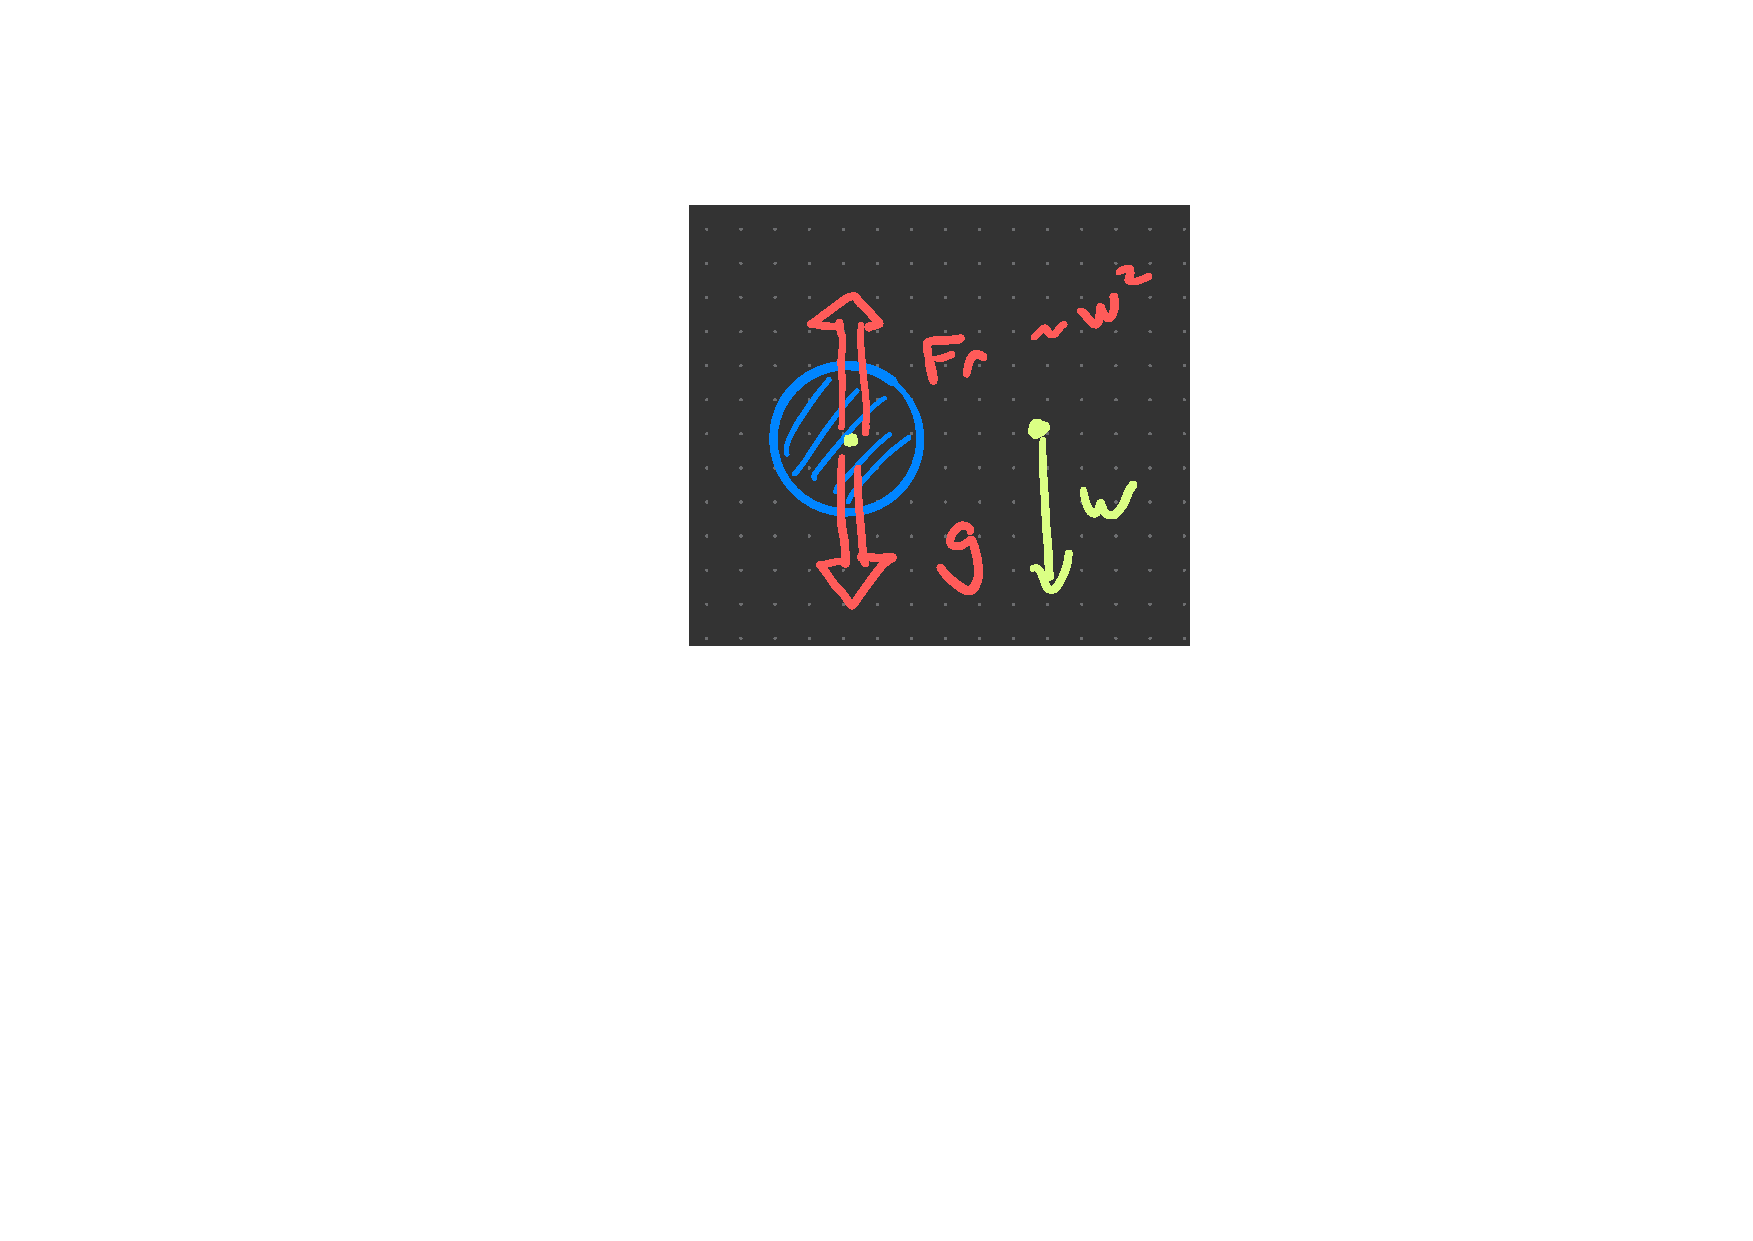
\includegraphics[width=1.7in]{figs/Coriolis/TermVel}
    \caption{Sketch of terminal velocity force balance.  In balance, the gravity force $g$ is equal and opposite to the friction force ($F_r$).}
    \label{fig:TermVel}
\end{marginfigure}

Newtons laws of motion apply to an \Wikiref{inertial reference frame}, i.e. a reference frame that is not accelerating.  An east way to think about this is to consider a cup of coffee on the dashboard of your car.  If you are travelling a constant speed, the coffee travels with your dashboard and there are the only forces on it are vertical (gravity and the normal force, \fref{fig:SketchApparent}, left-top).  Now suppose the car accelerates with acceleration $a$.  From an outside observer's point of view, the cup continues to move at the same speed, but the car starts to accelerate away from the coffee cup (\fref{fig:SketchApparent}, left-middle sketch). However, if you are sitting in the car, it is like a force pushed the cup so that it accelerates towards the back of the car (\fref{fig:SketchApparent}, left-bottom sketch). This would be an \Wikiref{apparent force} in the accelerating reference frame of the car.


\begin{figure}[hbt]
  \begin{center}
  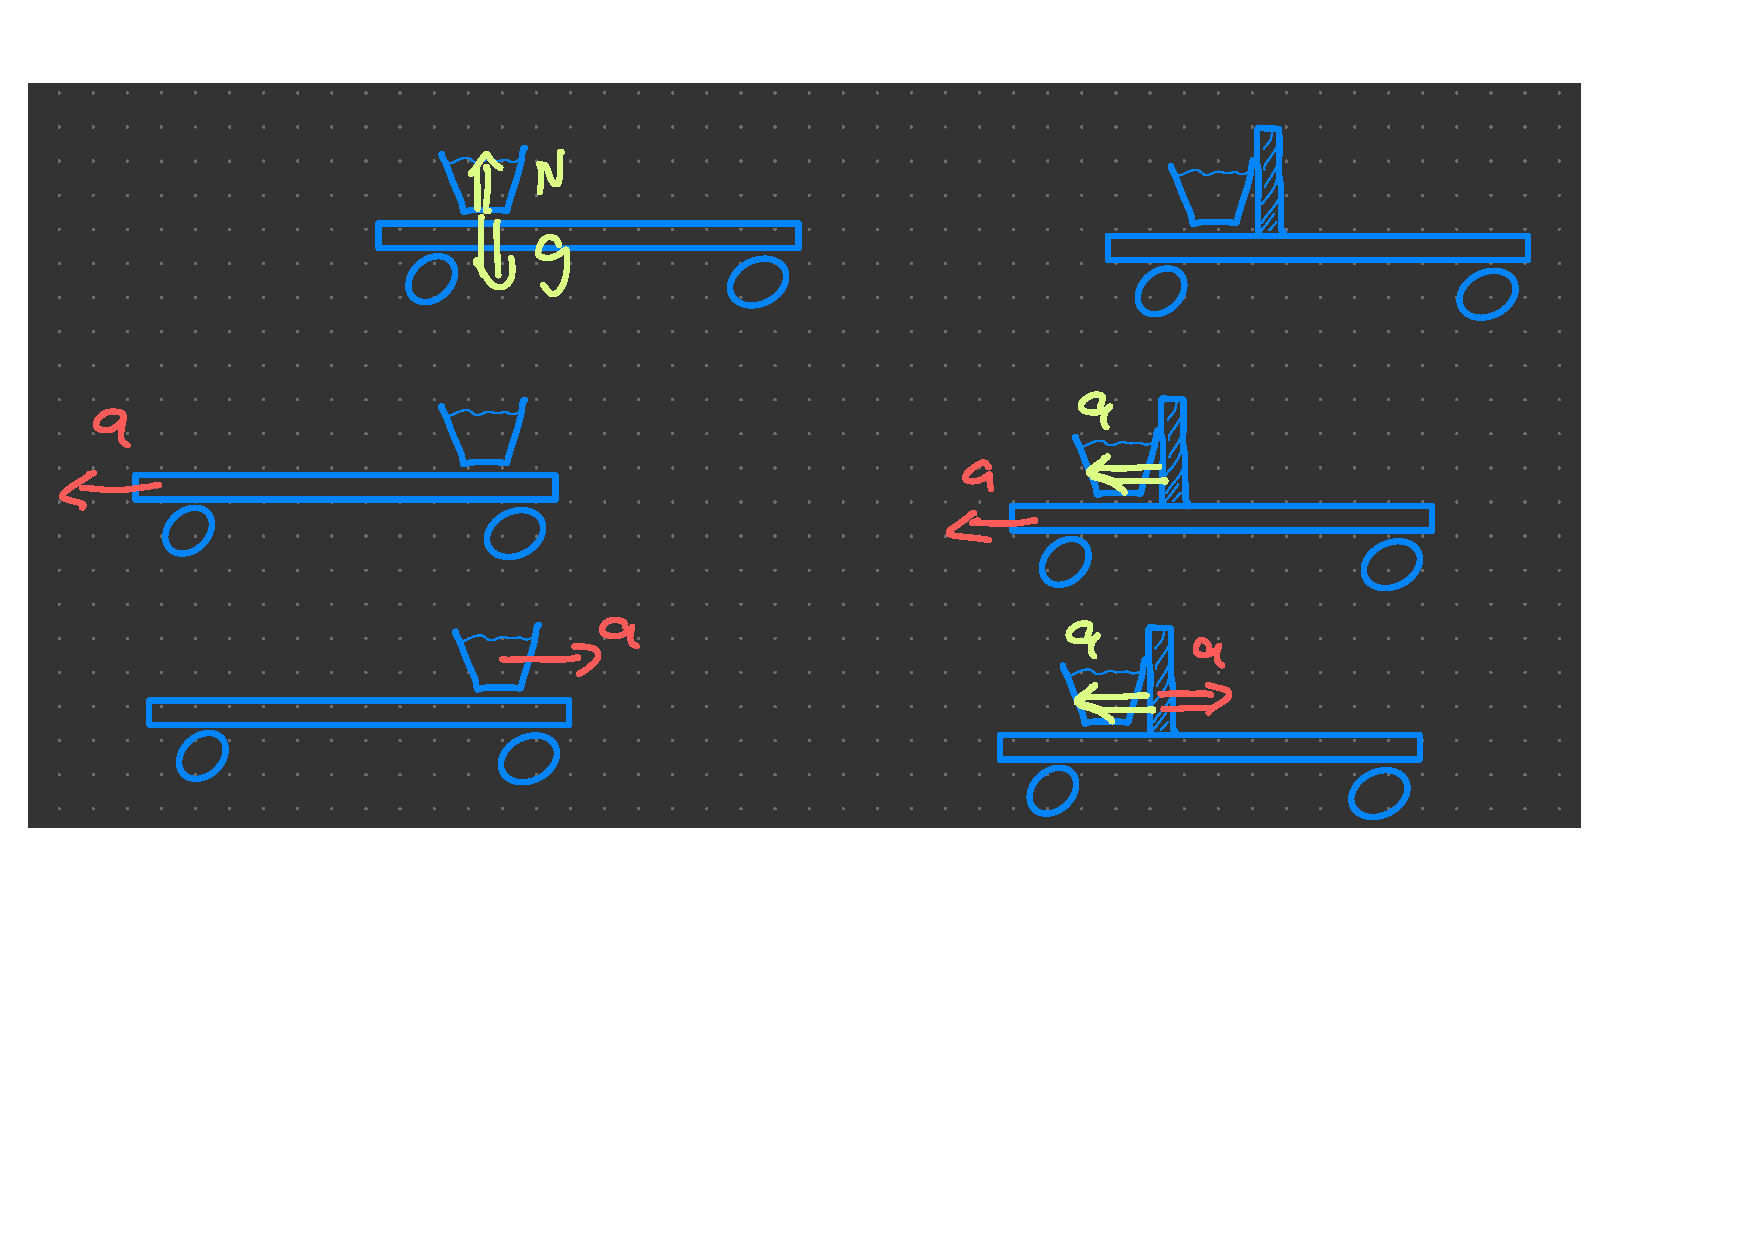
\includegraphics{figs/Coriolis/SketchApparent}
    \caption{Apparent force on a cup in a car.  Left side are frictionless cups (or a ball if you prefer) on an accelerating car.  Right hand side is a cup held laterally by a cup holder.}
    \label{fig:SketchApparent}  
  \end{center}
\end{figure}

If the cup moves with the car, then something has to supply a lateral force to cause that acceleration.  So, imagine a wall that the coffee can push against, or a cupholder (\fref{fig:SketchApparent}, top-right).  From an outside observers point of view, there is only one force acting on the cup, $a$ to the left supplied by the cup holder, accelerating the cup at the same rate the car is being accelerated.  However, someone inside the car may very well feel that there is a force pushing the cup to the back of the car, and infer an equal-and-opposite force towards the front, so the cup does \emph{not} accelerate in this frame of reference.  

Hopefully this change of reference frames makes sense to you.  If you are sitting in a car and the driver slams on the brakes, you don't say that you were "slowed down more slowly than the car", you say that you were ``thrown forward''.  Of you accelerate very quickly, you say you were ``pushed back in your seat''.  

The application to the earth is hopefully obvious - the earth is constantly rotating, and hence any point rotating with the earth is constantly changing its velocity (but not its speed!), and hence the rotating frame is not an inertial frame of reference.  

\section{Centrifugal and Coriolis forces}

 A rotating reference frame gives rise to \emph{two} apparent forces, the \Wikiref{centrifugal force} and the \Wikiref{Coriolis force}.  The centrifugal force is felt everywhere on the planet and is a constant that depends on position, so we actually roll it into our definition of gravity and promptly forget about it (except perhaps on an exam).  The Coriolis force only arise if a body is moving relative to the rotating frame.  
 
 In oceanography, when we say a parcel of water moves at 1 m/s, it is doing so in the rotating frame.  From space it is moving at 132 m/s (at 49 N), where most of that is the earth's rotation.  Doing everything from a frame that is out in space is possible, but extremely awkward!
 
 \subsection{Centrifugal force}

\begin{marginfigure}
    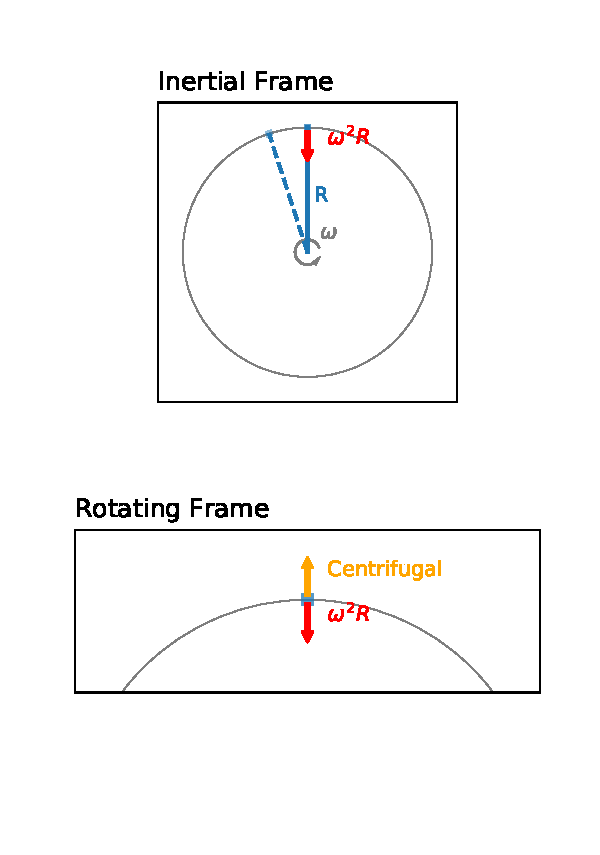
\includegraphics{figs/Coriolis/CentrifugalForceCor}
    \caption{Forces on a rotating reference frame observed from an inertial reference frame (i.e. from space).  There needs to be a centripetal force applied to any object going around the circle or it will be flung off the orbit.  An observer in the rotating frame sees two forces: the centripetal force and an apparent centrifugal force that works against the centripetal force to keep the body in place on the rotating frame.}
    \label{fig:CentrifugalForceCor}  
\end{marginfigure}

 
The earth spins about its axis every 24 h, such that it spins counter clockwise when looking down on the north pole.  Because this is an important constant it gets a capital $\Omega = 2\pi/24h =7.27\times10^{-5}\ \mathrm{rad\,s^{-1}}$.  The radius of the earth is $R=6731 \ \mathrm{km}$, and the radius at any given latitude $\lambda$ is given by $r = R\cos(\lambda)$.  As pointed out in \fref{box:centrifugalforce}, the linear speed of a particle is given by $\omega r$ and the velocity is tangential to the circle.  The acceleration needed to keep going in a circle is readily shown to be $a_c = r \omega^2$.  A mass on the rotating system that suddenly becomes unglued will be flung away from the axis of rotation, and we call this the \Wikiref{centrifugal force} (\fref{fig:CentrifugalForceCor}).

So, as you sit in you chair (or comfy sofa) reading this, what keeps you rotating around the axis of the earth's rotation?  There needs to be a centripetal force to counteract the centrifugal force that wants to fling you into space.  This force, at 49 degrees of latitude is 
\begin{equation}
    a_{cent} = R\cos\left(\lambda\right)\ \omega^2 = 0.0107 \ \mathrm{m\,s^{-2}}    
\end{equation}
so its small compared to gravity, but is not non-zero.  You may argue that it is friction with your chair that keeps you in place, but that doesn't apply if your chair has wheels, or to a hockey puck on an ice rink.  The answer is that the earth is not a sphere, and bulges out at the equator, precisely because it is spinning; the equatorial radius is 22 km more than the polar radius. 

This leads to a centripetal force because there is an imbalance between the normal force exerted by the earth's spheroidal surface and the direction that gravity points.  First, consider the forces on a body sitting on a perfect sphere as observed from an inertial frame (i.e. space; \fref{fig:CentrEarth} left panel).  There are two real forces acting on the body - gravity pulls towards the center of the earth, and there is a normal force due to the body of the earth that pushes back.  Because this is a perfect sphere the normal force is in the same direction as the gravity force, pointing away from the center of the sphere.  Combined, then there are no net forces on the object, and hence the object will \emph{not} orbit with the spinning of the earth.  

\begin{figure}[hbt]
  \begin{center}
    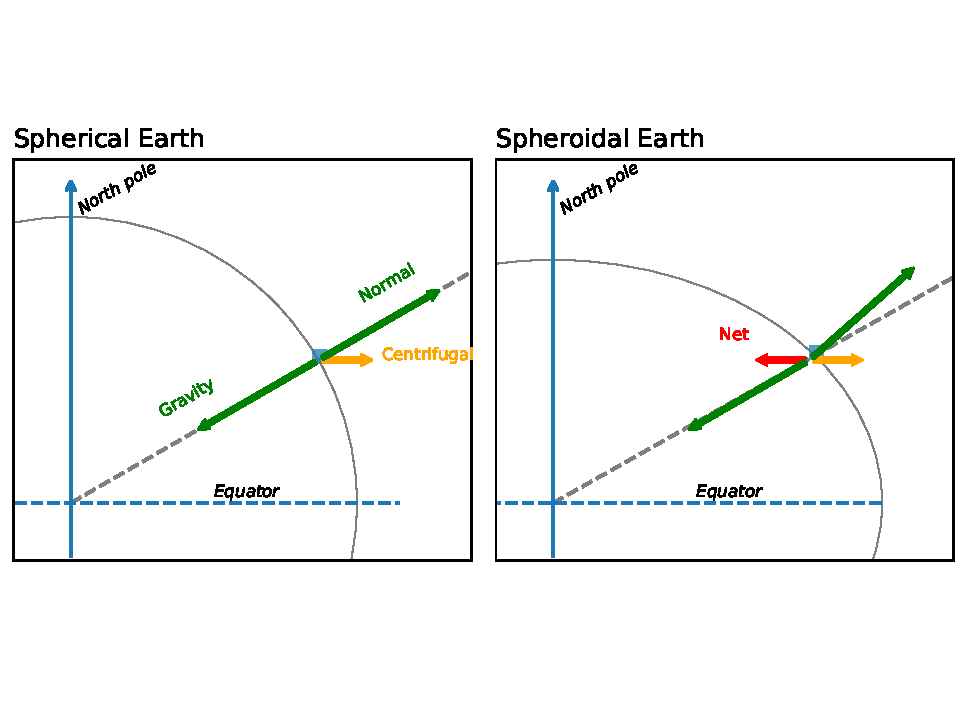
\includegraphics{figs/Coriolis/CentrEarth}
    \caption{Left panel: forces on an object on a perfect sphere.  There is a normal force that is exactly equal and opposite to the gravity force because the normal on a perfect sphere points towards the centre of the sphere.  Right panel: the same forces on an oblate spheroid; the normal force and the gravity force are at angles to one another leading to a net force towards the axis of rotation.}
    \label{fig:CentrEarth}  
  \end{center}
\end{figure}

Naturally, this does not happen on the real earth - if somehow we started with a spinning perfect sphere earth it would tectonically shear apart until it made a bulge at the equator that balanced the spinning.  Such a  bulge is in rotational equilibrium when the normal force at any point on its surface points at an angle to the center of the earth so that the sum of the two forces result in a net force towards the axis of rotation (\fref{fig:CentrEarth}, right panel). The faster a planet spins, the larger this bulge is.  Of course there are irregularities on a real planet, like mountains, but if you put your chair on the mountain side, you would roll off.  

Now consider a plumb bob hanging above the surface of the earth.  It is \emph{not} just pulled down towards the center of the earth, but also is flung out slightly by the centrifugal acceleration. Hence it will fall parallel to the normal line in \fref{fig:CentrEarth}, (right side), and not towards the center of the earth. Hence we call this direction "down" and "up" and we slightly modify the value of gravity to account for the centrifugal acceleration.  Hence you will find gravity calculators that depend on the latitude $\lambda$.  

\subsection{Coriolis force}

The \Wikiref{Coriolis force} is the second apparent force in a rotating reference frame.  It only occurs if the object has a velocity relative to the rotating frame. It is quite unintuitive, and has no easy analogue like in the accelerating car.  i.e. the cup feels the same acceleration whether it is already moving in the car or not.  

The Coriolis force acts exactly 90 degrees to the right of the velocity vector in the Northern hemisphere, and to the left in the Southern. The strength of the force is linearly proportional to the velocity: 
\begin{equation}
    |\mathbf{F_{Coriolis}}| = f |\mathbf{u}| \ \ \ \mathrm{to\ the\ right\ of\ \mathbf{u}} 
\end{equation}

Understanding how this force arises is not terribly difficult (and the math is even easier if you know some vector calculus).  First, consider a hockey player shooting a puck along a frictionless ice rink.  That person is rotating on the earth, and hence is being pulled into the center of the earth by the net centripetal acceleration (\fref{fig:ThrowerMotion}).  You can think of this as the summation of two vectors, the tangential motion of the hockey player at travelling a distance $\omega r\ \delta t$, and the motion towards the axis of rotation $0.5\omega^2 r \ \delta t^2$.  

\begin{figure}[hbt]
  \begin{center}
    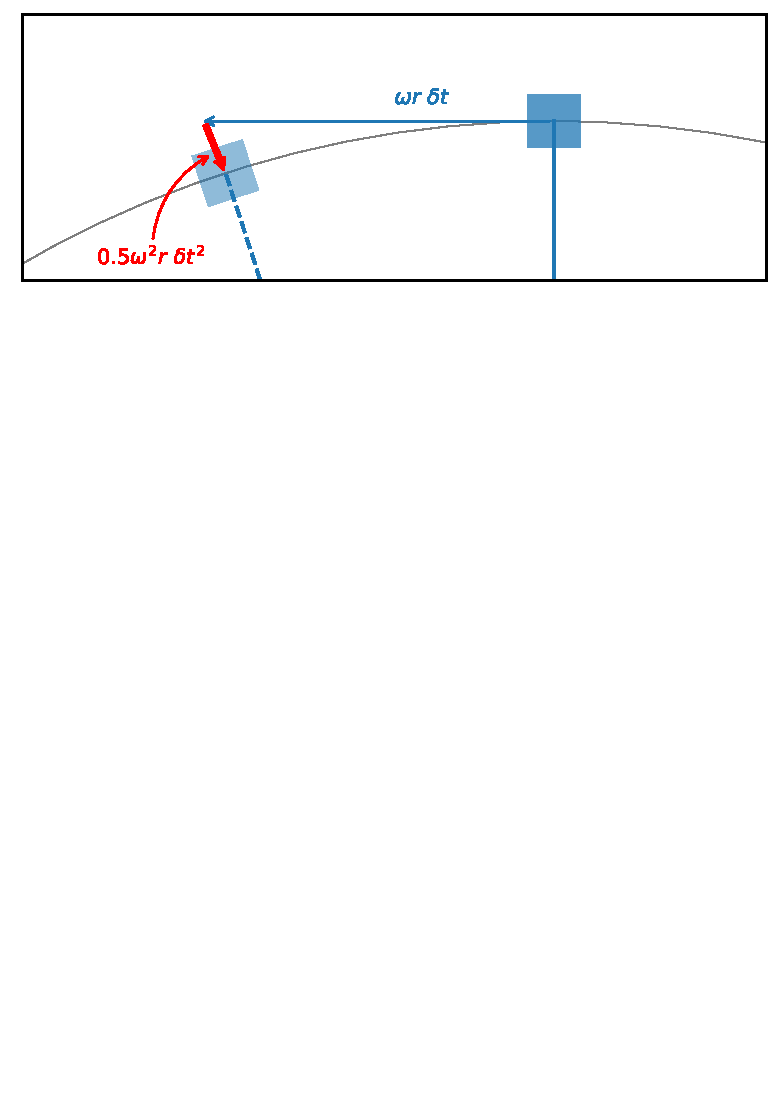
\includegraphics{figs/Coriolis/ThrowerMotion}
    \caption{Forces on a person who is stationary in the rotating frame. }
    \label{fig:ThrowerMotion}  
  \end{center}
\end{figure}

Now, suppose they aim the puck away from the axis of motion, which on the northern hemisphere is like aiming at a target to the south (\fref{fig:SouthSetup}).  Note that the target moves further to the left than the hockey player, and then is pulled back into orbit by a stronger centripetal force because it is further from the axis of rotation. The hockey player shoots the puck with enough velocity to hit the target, and the aim directly away from the axis of rotation.  

\begin{figure}[hbt]
  \begin{center}
    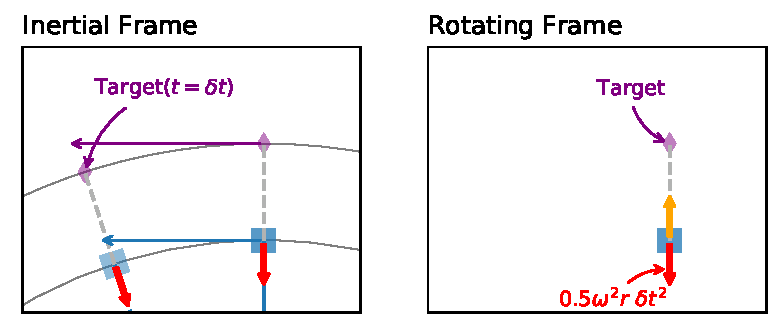
\includegraphics{figs/Coriolis/SouthSetup}
    \caption{Left panel: forces in the inertial frame of a hockey player aiming at a target further from the axis of rotation. Note that the target has a \emph{faster} tangential velocity than the hockey player.  Right panel: setup in the rotating frame observed by the hockey player.  }
    \label{fig:SouthSetup}  
  \end{center}
\end{figure}

What happens when the player shoots the puck is that everything continues to rotate because of the centripetal force, but the puck does not have enough tangential velocity to hit the target.  In \fref{fig:SouthThrow}, the puck ends up at the summation of three vectors - the first two are (ahem, almost) the same as the hockey players, the tangential distance $\omega r\ \delta t$, and the motion towards the axis of rotation $0.5\omega^2 r \ \delta t^2$. The third is the velocity component $U\ \delta t$ imparted by the player when they shot the puck. Adding these three together, it should be clear that the puck can't keep up with the target, and ends up ``behind'' it, or to the right of the velocity (\fref{fig:SouthThrow}, Rotating Frame).  

\begin{figure}[hbt]
  \begin{center}
    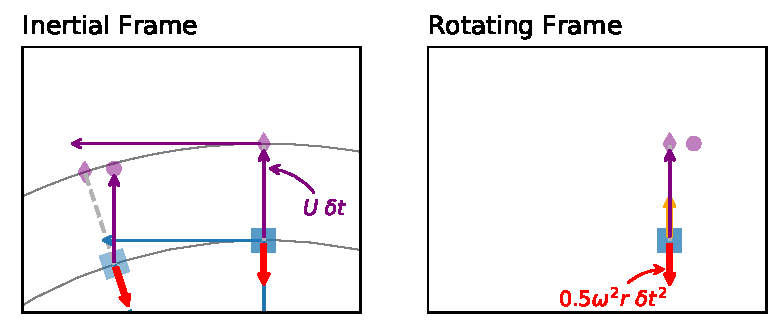
\includegraphics{figs/Coriolis/SouthThrow}
    \caption{Left panel: The result of the shot after a time $\delta t$ in the rotating frame, where the circle is the puck.  the puck doesn't have enough velocity to the ``left'' to keep up with the target and falls behind.   Right panel: in the rotating frame, the puck veers to the right of the target.}
    \label{fig:SouthThrow}  
  \end{center}
\end{figure}

Why does a greater velocity result in a greater Coriolis force?  Quite simply the puck would get further away from the axis of rotation in time $\delta t$, and would fall even further behind the new, more distant target.  
 
A similar effect happens if the throw is in the tangential direction.  In this case this would be to the ``east'' if the shot was taken in the Northern hemisphere.  In this case, the puck is given too much tangential velocity (\fref{fig:Response}).  It still gets pulled in towards the axis of rotation the same amount as the hockey player, but it has more tangential velocity so it ends up further from the axis of rotation.  The hockey player sees it fly to the right. 


\begin{figure}[hbt]
  \begin{center}
    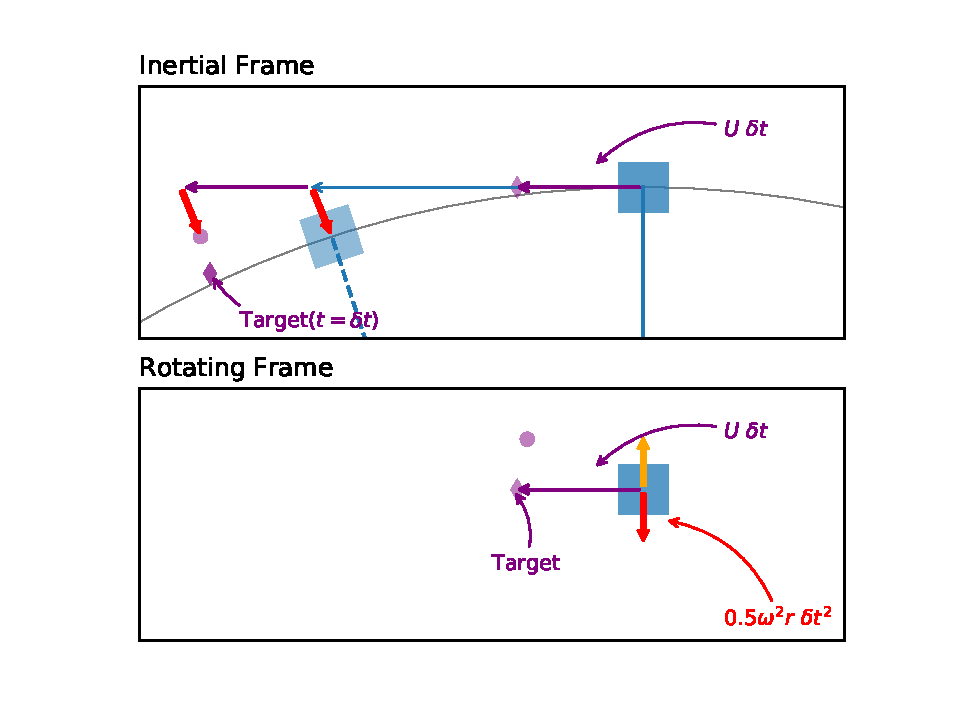
\includegraphics{figs/Coriolis/Response}
    \caption{Upper plot: a shot in the same direction as rotation.  The puck has (approximately) the same centripetal acceleration towards the axis of rotation, but has too much momentum to be pulled back to the original orbit, and hence moves in a net sense away from the axis of rotation.  Lower plot: as observed by the hockey player, the puck veers to the right of the target.}
    \label{fig:Response}  
  \end{center}
\end{figure}

the astute reader will note that the puck now has a component of velocity that has turned to the right of it original motion.  This should mean the Coriolis force turns to the right at the same time.  Indeed what happens is that the Coriolis force pushes the particle around a circle with a frequency given by the proportionality constant $f$.  This type of motion is regularly seen in the ocean (\fref{fig:inertial_currents}), and is called an \Wikiref{inertial oscillation}.

\begin{figure}[hbt]
  \begin{center}
    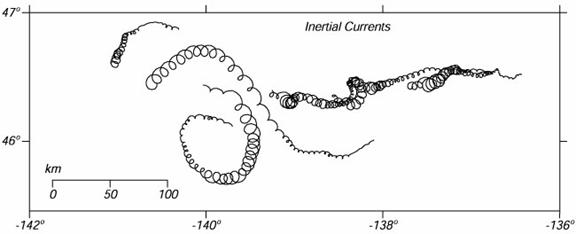
\includegraphics{figs/Coriolis/inertial_currents}
    \caption{Response of surface drifters in the ocean to a sudden windstorm.  Note the circular motion superimposed on the mean currents.}
    \label{fig:inertial_currents}  
  \end{center}
\end{figure}


It is interesting to note that the Coriolis force is the same \emph{everywhere} in the rotating reference frame, and depends only on the velocity and the angle of the velocity with the axis of rotation.  However, a the earth is a sphere, and we specify our velocities as horizontal velocities along the sphere (eastward: $u$, northward: $v$) and upwards perpendicular to the geoid ($w$).  Usually the Coriolis force due to motions in the vertical is very small ($w<<u$), so we only deal with the horizontal terms, but these make an angle to the axis of rotation everywhere on the sphere, except 
right at the poles.  That angle means that the horizontal component of the Coriolis force is $f = 2\Omega sin\lambda = 1.45\times10^{-4}\ \mathrm{rad\, s^{-1}}$, where $\lambda$ is the latitude.  So, $f=2\Omega$ at the north pole, $0$ at the equator, and $-2\Omega$ at the south pole.  At the mid latitudes ($\lambda=45^o \ N$) $f\approx10^{-4}\ \mathrm{rad\,s^{-1}}$.  

The minus sign in the southern hemisphere means that inertial motions are counter clockwise.  This is just because "up" points closer to the south pole than towards the north pole.  A puck pushed eastward in the southern hemisphere is still flung away from the axis of rotation, its just that away from the axis of rotation in the southern hemisphere means moving northward instead of southward.  You can also think of this as looking down at the earth spinning from the south pole, in which case it appears to turn clockwise and we can think of the rotation rate as being $-\Omega$.  

Mathematically, we write the horizontal equations of motion as 
\begin{eqnarray}
    \label{eq:motion}
    \frac{du}{dt} & = & +fv  - \frac{1}{\rho}\frac{dP}{dx} +  \sum F_{x}\\
    \frac{dv}{dt} & = & -fu - \frac{1}{\rho_0}\frac{dP}{dy} + \sum F_{y}
\end{eqnarray}
where $F_x$ and $F_y$ are the friction forces in x and y.  

\begin{derivbox}[label={box:nonlinear}]{Non-linearity of equations of motion}
The equations in \fref{eq:motion} are adequate for our needs, but note that these are the equations following a parcel of water, just like in classical mechanics how we would follow the forces on a single ball. In fluid mechanics we call this the \Wikiref{Lagrangian reference frame} and usually specify with a capital $D$ instead of lower case $d$ (i.e. $\frac{Du}{Dt}=...$).  

However, we usually cannot follow a parcel of water, so the derivatives at a point have terms that are due to the water moving from one point to another.  This is called the Eulerian reference frame, and is what makes water flow so complicated because there are nonlinear terms:
\begin{equation}
    \frac{Du}{Dt} = \frac{\partial u}{\partial t} + u\frac{\partial u}{\partial x} + v\frac{\partial u}{\partial y} + w\frac{\partial u}{\partial z}
\end{equation}
Including these terms makes mathematically solving the equations of motion very difficult!
\end{derivbox}


\section{Friction force}

Now we only need to consider the final terms in \fref{eq:motion}, the friction forces.  Friction forces are quite complicated in general, but lets consider a simpler flow.  Suppose there is a flow in the x-direction, and that it has \Wikiref{shear} in the vertical such that the faster flow is above the slower (\fref{fig:stress}).  Because the fluid is viscous, the faster flow above will exert a stress to the right on the flow below, and the slower flow will exert a stress to the left on the faster flow.  This will decelerate the upper flow and accelerate the lower flow (\fref{fig:Stress}).  This transfer of momentum occurs at a rate proportional to the shear and the viscosity of the fluid:
\begin{equation}
    \frac{\tau_{xz}}{\rho} = \nu \frac{du}{dz}
\end{equation}
where the subscript $xz$ means transfer of x momentum in the z-direction.  Here $\nu$ is the kinematic viscosity and has a molecular value of $\nu \approx 10^{-6}\ \mathrm{m^2\,s^{-1}}$.  Note that the units are the same as for a diffusion co-efficient, and can be thought of as a diffusion of x-momentum in the vertical. 

\begin{figure}[hbt]
  \begin{center}
    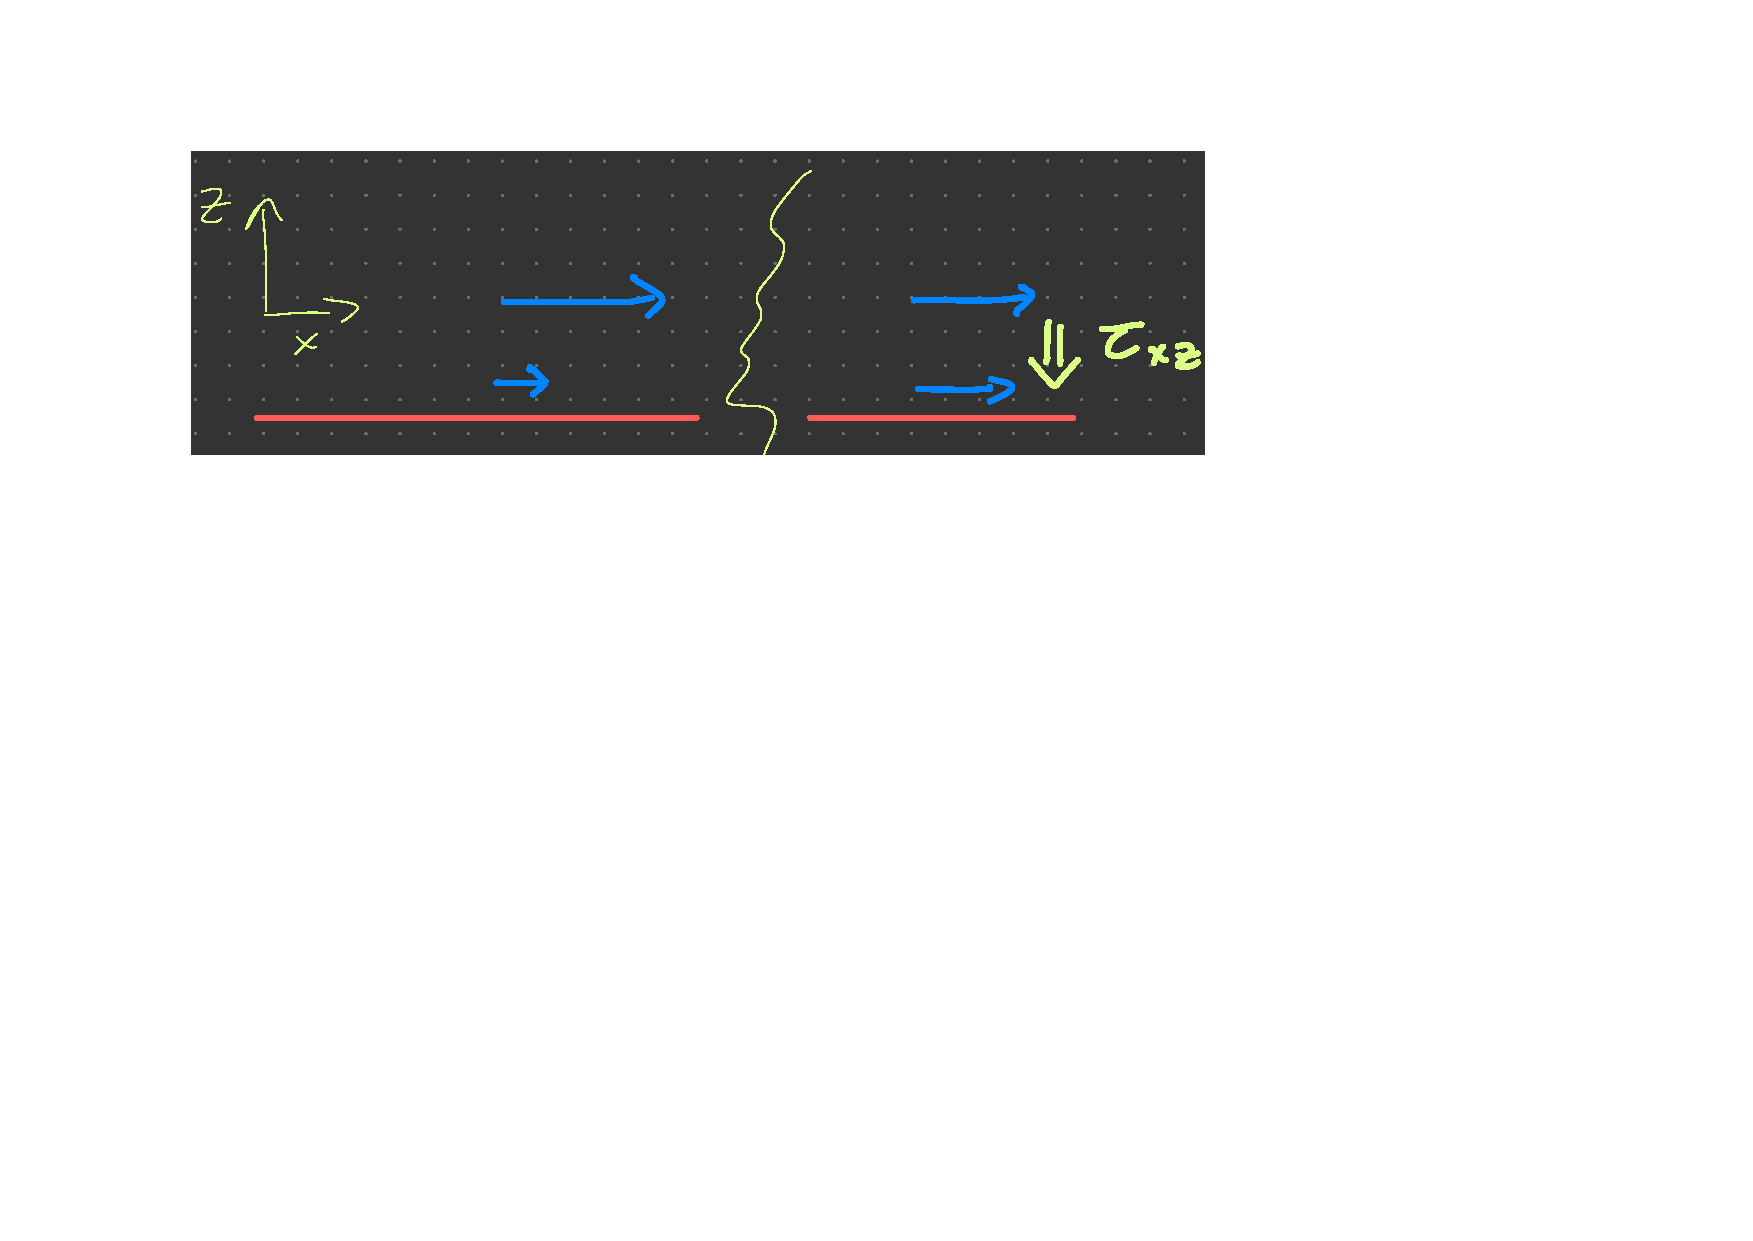
\includegraphics{figs/Coriolis/Stress}
    \caption{Left: Velocity in x-direction with faster flow above slower (blue arrows). Right: velocity after there has been a downward transfer of x-momentum ($\tau_{xz}$); the faster velocity has slowed, and the slower velocity accelerated.}
    \label{fig:Stress}  
  \end{center}
\end{figure}

The net force at any point depends on the difference of the stresses in the vertical (\fref{fig:NetStress}).   The parcel gains momentum from above, but loses it below.  So in this simplified flow 
\begin{equation}
    F_x = \frac{1}{\rho}\frac{d\tau_{xz}}{dz}+ other\ friction\ in\ x = \nu \frac{d^2u}{dz^2} + other\ friction\ in\ x
\end{equation}
So just like for diffusion,  the flow needs to have some curvature ($\frac{du}{dz} \neq 0$) for there to be a net effect on the velocity due to friction.  

\begin{figure}[hbt]
  \begin{center}
    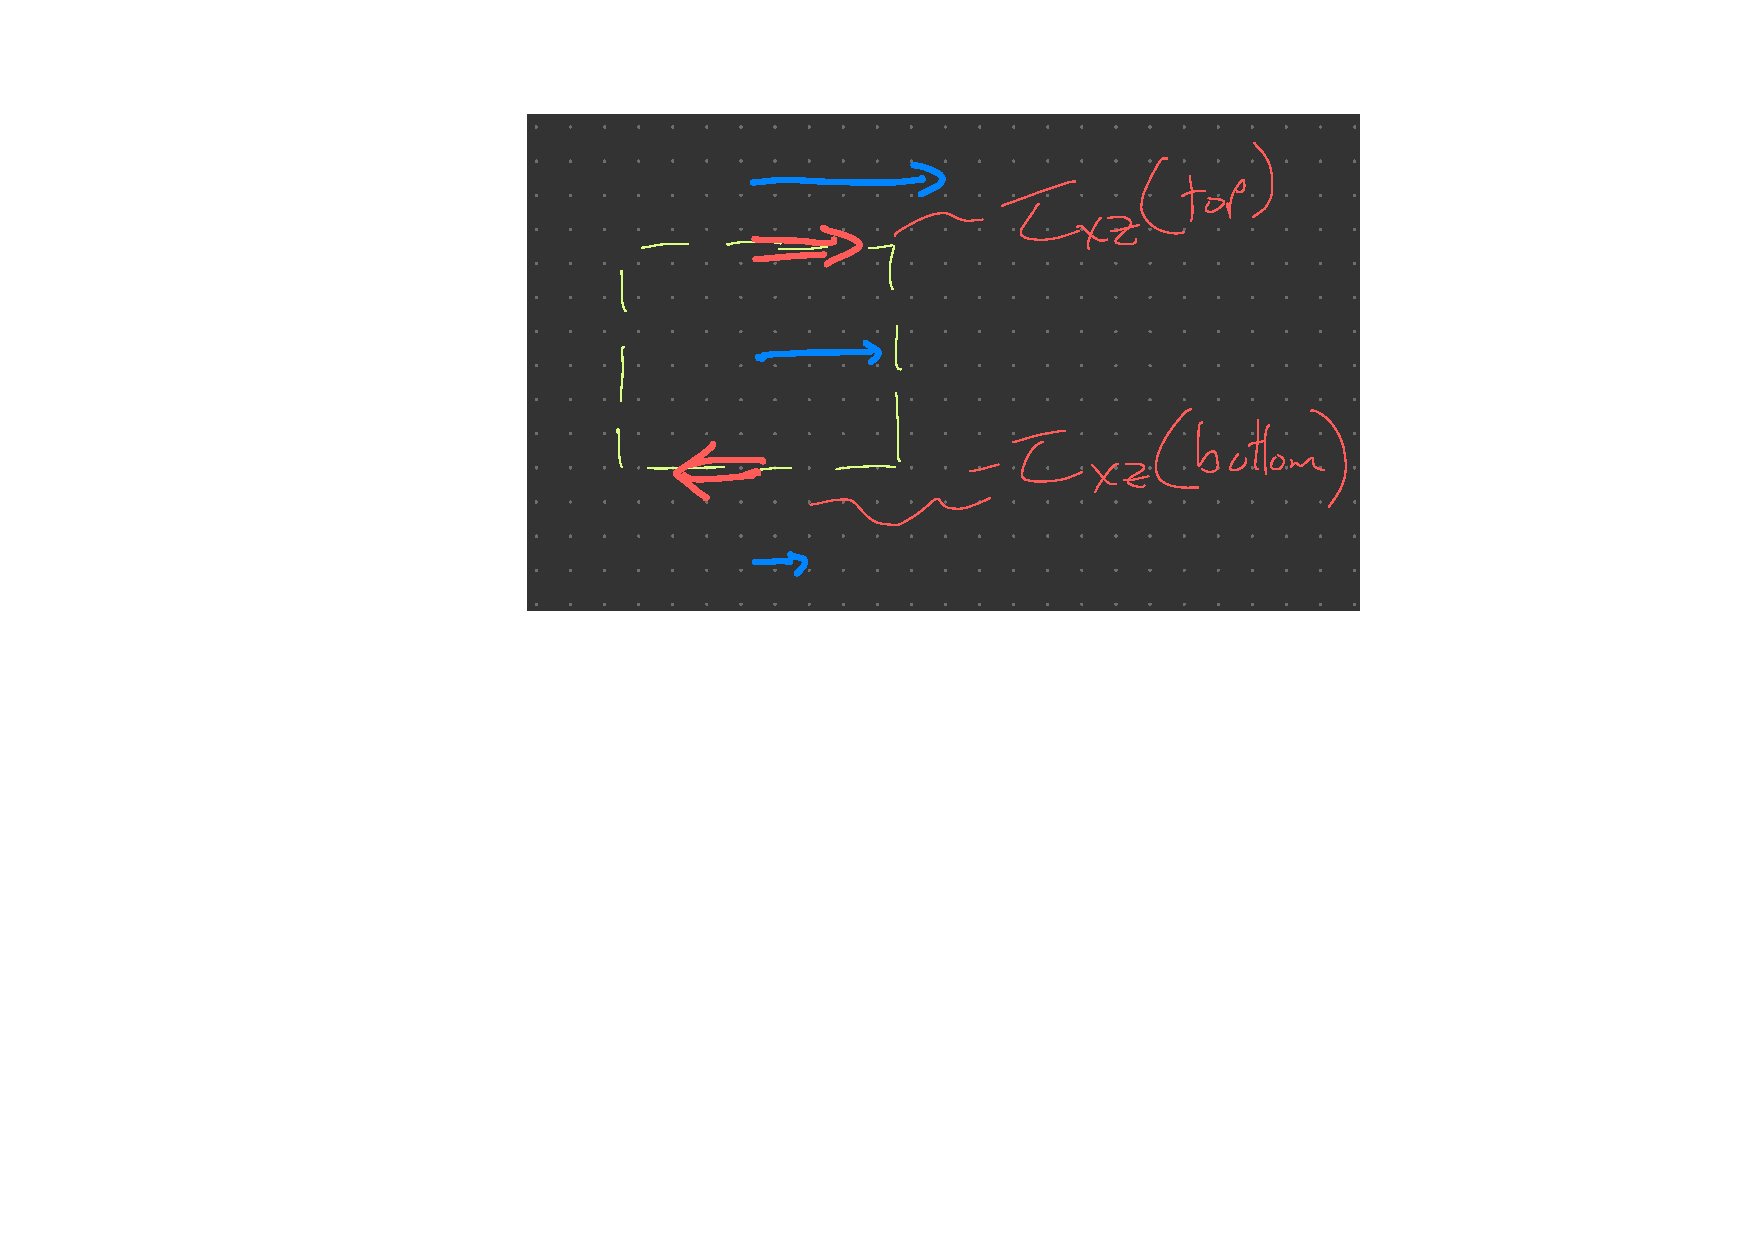
\includegraphics{figs/Coriolis/NetStress}
    \caption{Net stress on a parcel (yellow dashes) in a sheared flow (blue velocity arrows) is the difference in the stress from top to bottom (red arrows).  The water above speeds up the parcel, but the water below slows it down.}
    \label{fig:NetStress}  
  \end{center}
\end{figure}

X-direction momentum doesn't just diffuse in the vertical direction.  If we re-drew \fref{fig:Stress} with $y$ replacing $z$ the same physics would apply, and similarly in the x-direction, so the full value of of the friction in x is:
\begin{equation}
    F_x = \frac{1}{\rho}\left(\frac{d\tau_{xz}}{dz} + \frac{d\tau_{xy}}{dy} + \frac{d\tau_{xx}}{dx}\right)
\end{equation}
and similar equations apply for $F_y$ and $F_z$, leading to nine total terms.  

\subsection{External stresses}

Water can have one of two boundary conditions - constant velocity (usually not moving), or constant stress.  Constant velocity means that at the boundary the fluid moves with the boundary, and is usually applicable to solid boundaries.  

Constant stress is often applied at the air-sea boundary as a ``wind stress''.  As the wind blows over the top of the ocean, it imparts some momentum to the ocean (and vice-versa).  We usually use the  symbol $\tau_x^w$ for the x-direction wind stress and $\tau^w_y$ where it is understood that the stress is being transmitted vertically.  

\begin{figure}[hbt]
  \begin{center}
    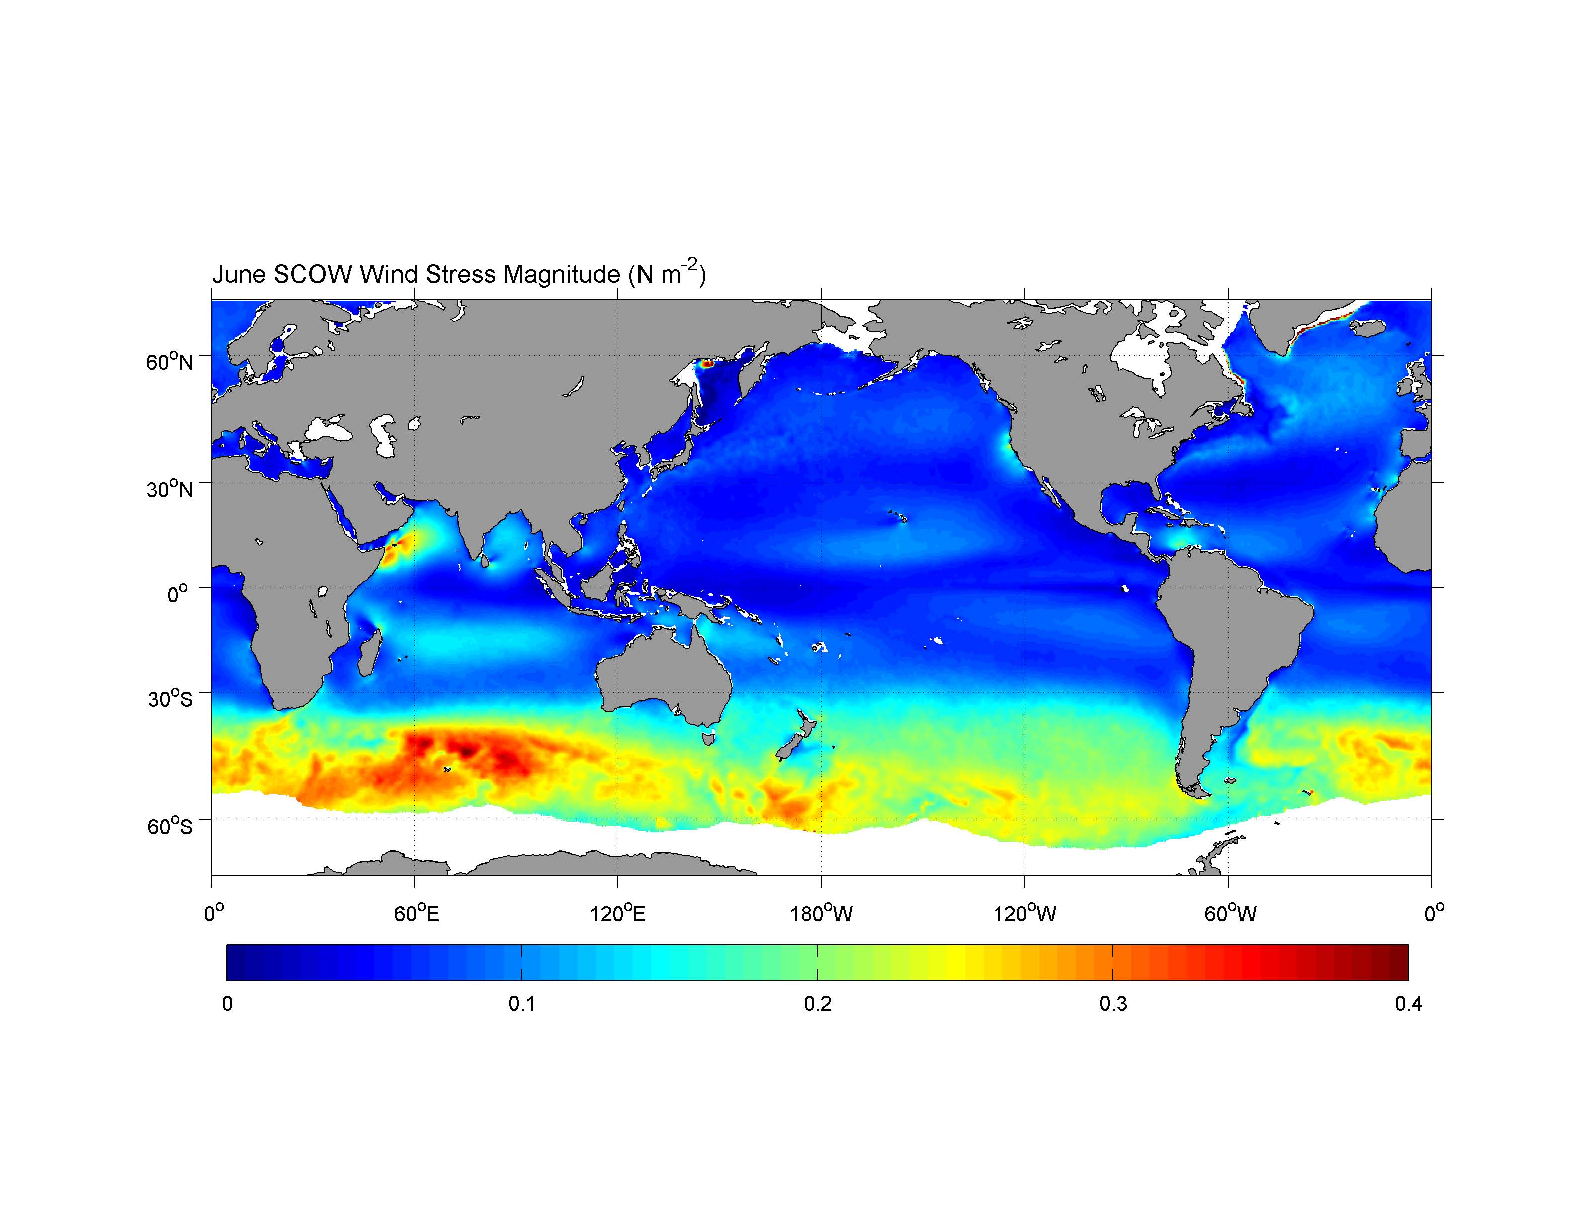
\includegraphics[trim=50 140 50 120,clip]{figs/Coriolis/June_SCOW_Wind_Stress_Magnitude-crop}
    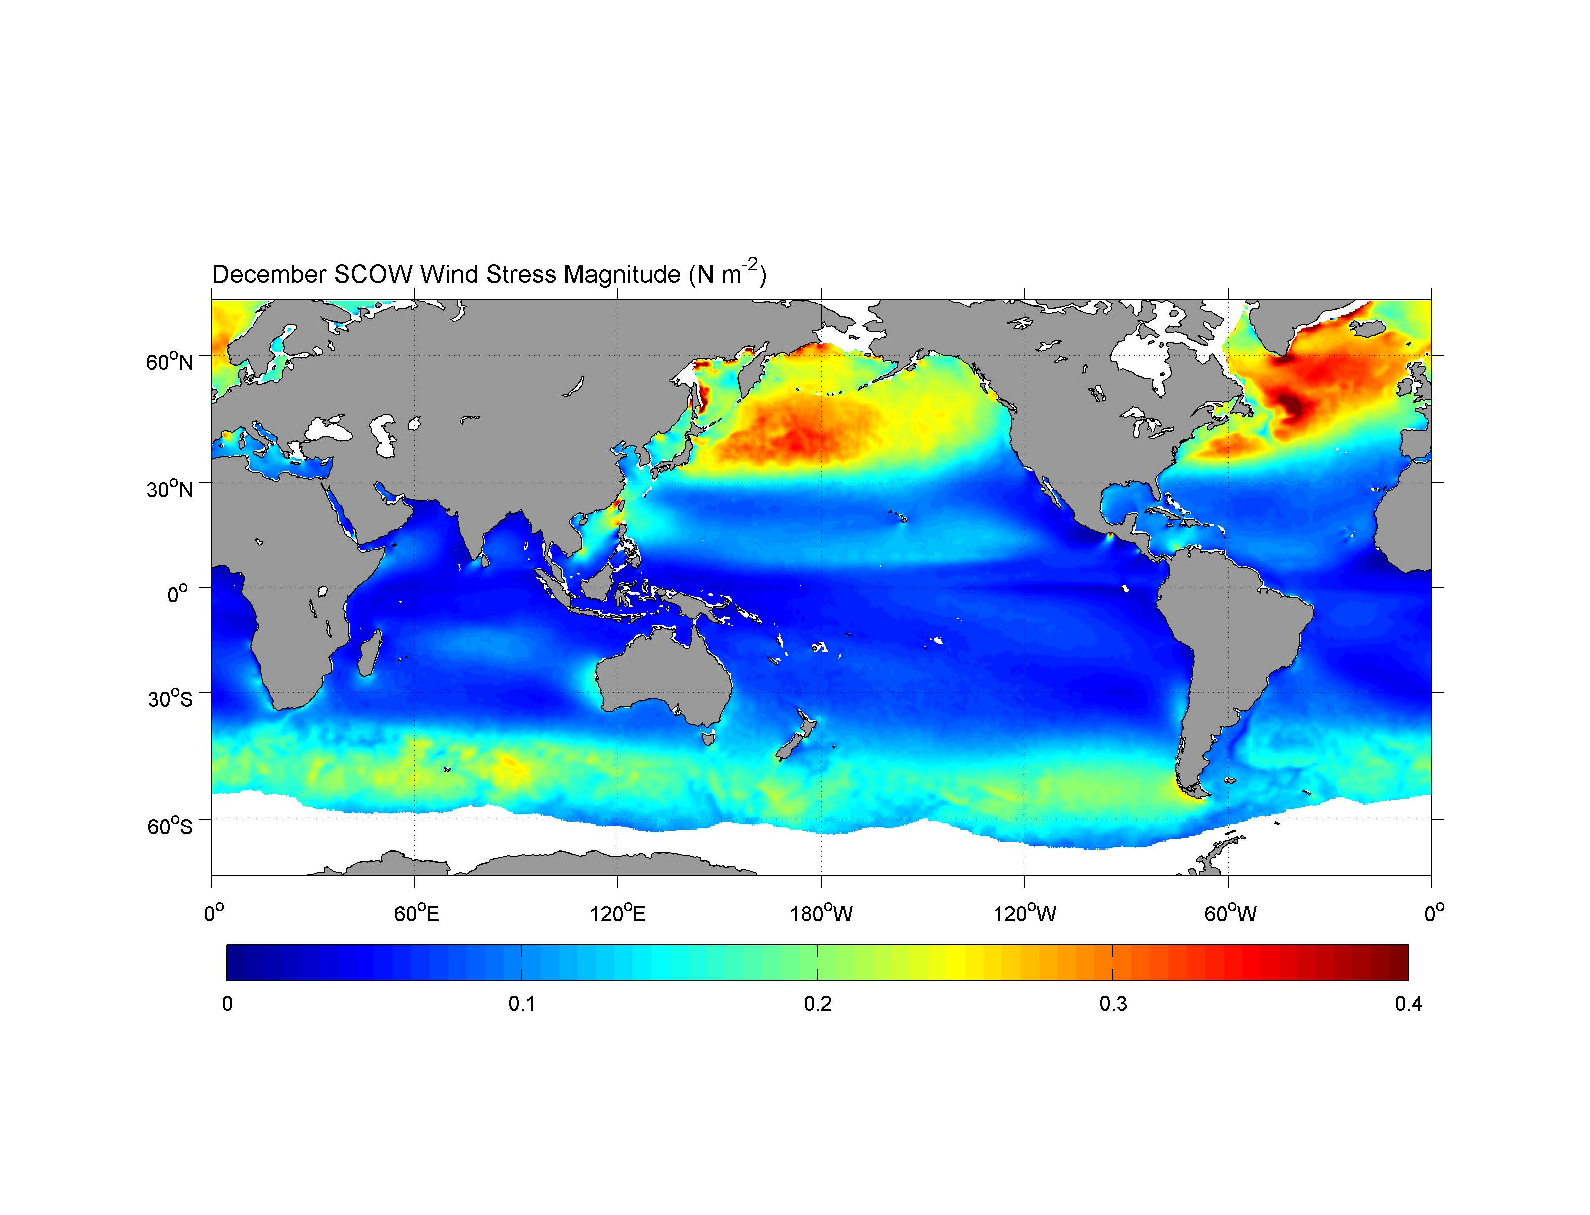
\includegraphics[trim=50 90 50 120,clip]{figs/Coriolis/December_SCOW_Wind_Stress_Magnitude-crop}
%    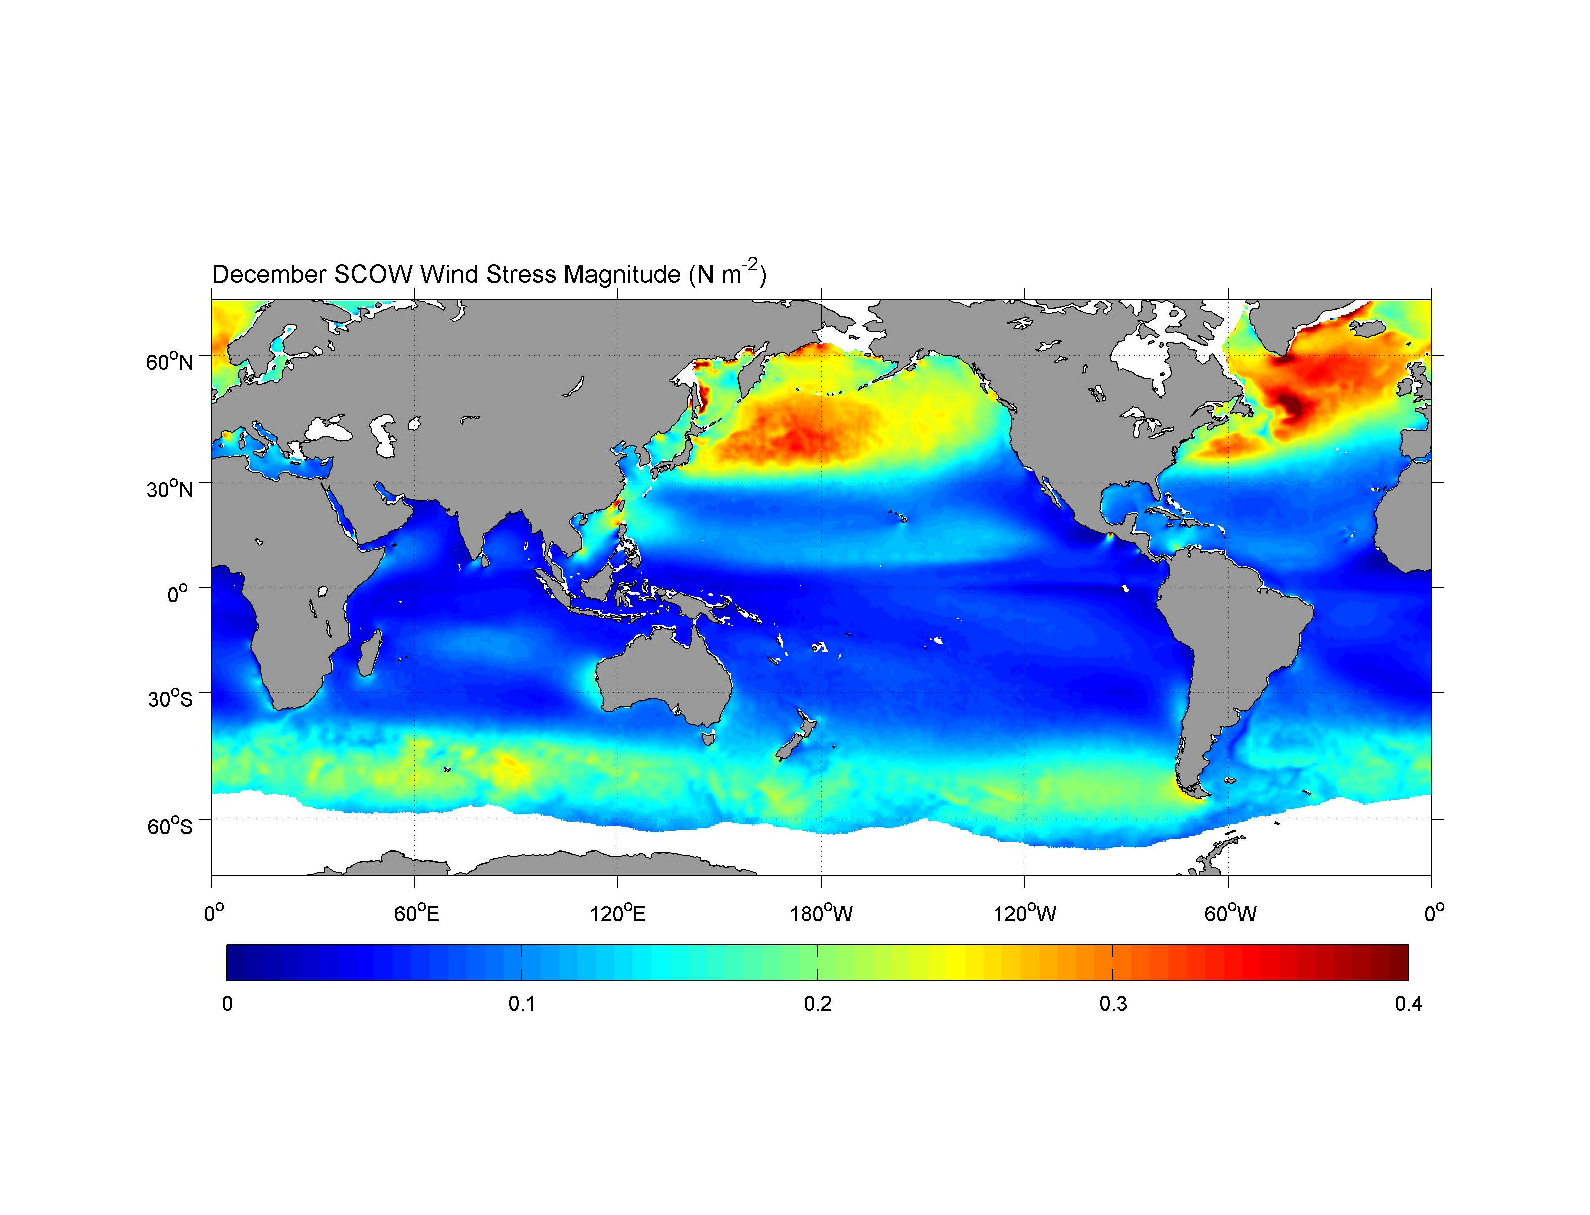
\includegraphics[trim=1200 400 1500 1500,clip]{figs/Coriolis/December_SCOW_Wind_Stress_Magnitude-crop}
  \caption{Wind stress amplitude, averaged for June and December.}
    \label{fig:Windstresses}  
  \end{center}
\end{figure}



\section{Ekman balance}
\label{sec:Ekman}

In physics it is often helpful to determine if a steady state exists.  In physical oceanography this means times when $du/dt=0$.  We saw in the previous chapter that the flow in the large-scale ocean actually \emph{does} change relatively slowly, so on long time scale this is approximately true.  Even in the coastal flow, the flow evolved slowly enough that the dominant balances are obeyed.  There are two such balances. The Ekman balance is  between the Coriolis and friction and friction forces, and the \Wikiref{Geostrophic balance} is between Coriolis and the pressure gradient force: 
\begin{equation}
    \frac{du}{dt} = \overunderbraces{\br{2}{geostrophic}}
    {- \frac{1}{\rho_0}\frac{dP}{dx} & +fv & + \frac{1}{\rho}\frac{d\tau_{xz}}{dz}}
    {&\br{2}{Ekman}}
\end{equation}
\begin{equation}
    \frac{dv}{dt} = \overunderbraces{\br{2}{geostrophic}}
    {- \frac{1}{\rho_0}\frac{dP}{dy} & -fu & + \frac{1}{\rho}\frac{d\tau_{yz}}{dz}}
    {&\br{2}{Ekman}}
\end{equation}
Here we discuss the first of these two balances, the Ekman balance.

The Ekman balance typically occurs near the boundaries where the shear stresses in the ocean are the largest.  In this region we assume that the friction is balanced by the Coriolis force, and ignore the pressure gradient force:
\begin{eqnarray}
   \frac{1}{\rho} \frac{d\tau_{xz}}{dz} & = & -fv\\
    \frac{1}{\rho}\frac{d\tau_{yz}}{dz} & = & -fu
\end{eqnarray}
The stress profile can be complicated, but if we integrate from some depth where $\tau_{xz}=0$, say at $z=-D$ to the sea surface, then we can write:
\begin{eqnarray}
    \frac{1}{\rho}\tau_x^w & = & -f\overline{v}D\\
    \frac{1}{\rho}\tau_y^w & = & f\overline{u}D
\end{eqnarray}
where $\overline{u} = \frac{1}{D}\int_{-D}^0 u\ \mathrm{d}z$ is the average velocity in the surface layer (same for $\overline{v}$).  In the coastal upwelling example, $D\approx20\ \mathrm{m}$ is probably appropriate, because that is the region where the turbulence is enhanced.  The terms $\overline{v}D$ and $\overline{u}D$ are called the Ekman transport and represent a 2-D transport with units of $\mathrm{m^2\,s^{-1}}$. 

So, for example in the coastal upwelling case, the wind is blowing from north to south, so the net force on the upper ocean is to the south (\fref{fig:EkmanLayerForces}).  If this force is in balance with the Coriolis force, then the Coriolis force must be towards the north.  Since the Coriolis force is to the north, that means there must be a net flow to the west (assuming this is northern hemisphere).  The other way to remember this is that the Ekman transport is to the right of the stress.  

\begin{figure}[hbt]
  \begin{center}
    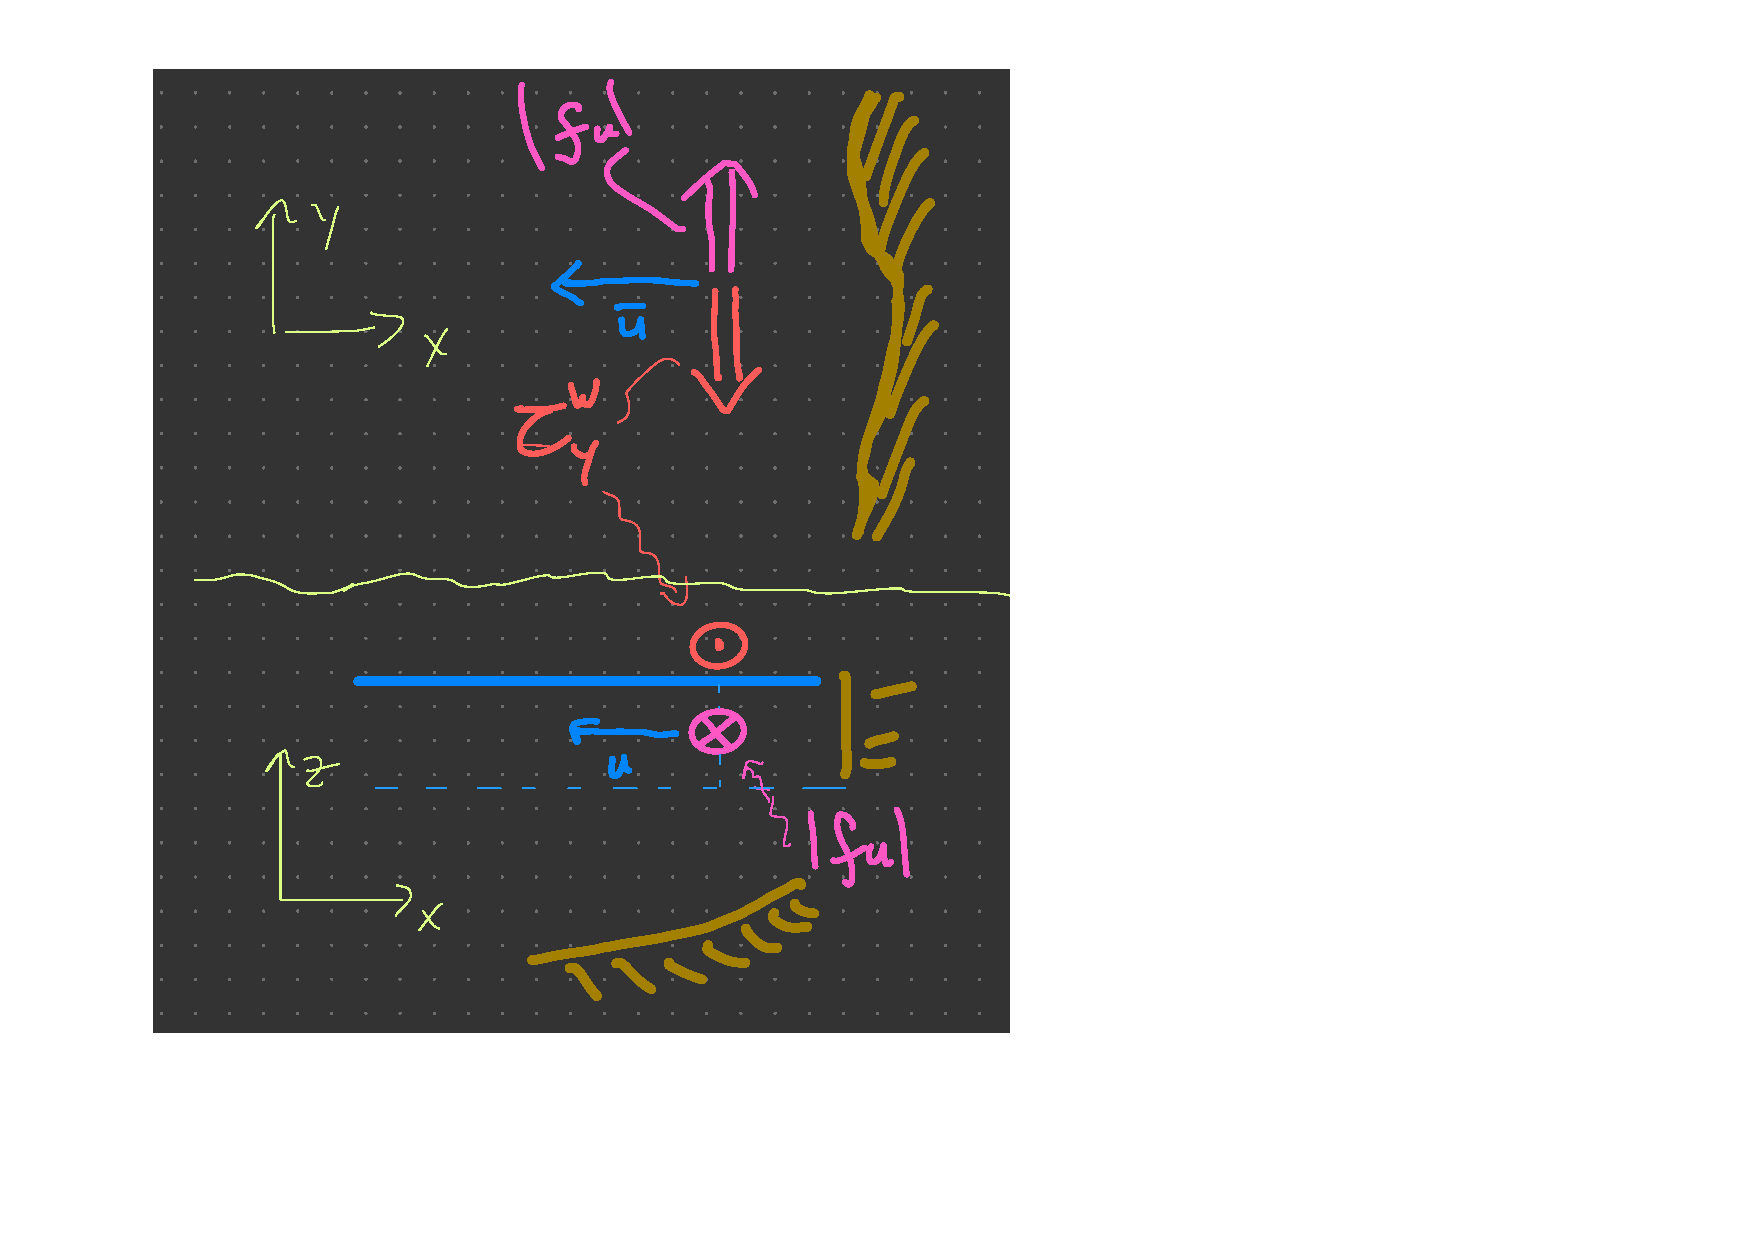
\includegraphics[width=3in]{figs/Coriolis/EkmanLayerForces}
    \caption{Sketch of the depth-integrated force balances in the Ekman layer in the coastal-upwelling case. Upper is looking from above, and lower sketch is looking from the south. }
    \label{fig:EkmanLayerForces}  
  \end{center}
\end{figure}

Stress can also be exerted at the sea floor by friction of the mean flow with the bottom.  Suppose, as in the coastal circulation example, the flow is towards the south.  Then there will be a friction to the north tending to slow this flow down, which we represent as a bottom stress $\tau_y^B$.  We saw in the observations that there is indeed heightened turbulence near the sea floor.  This also results in an Ekman layer, but now the stress is to the north (\fref{fig:EkmanBottomForces}), so the Ekman transport $\overline{u}D$ is to the east, or onshore.  

\begin{figure}[hbt]
  \begin{center}
    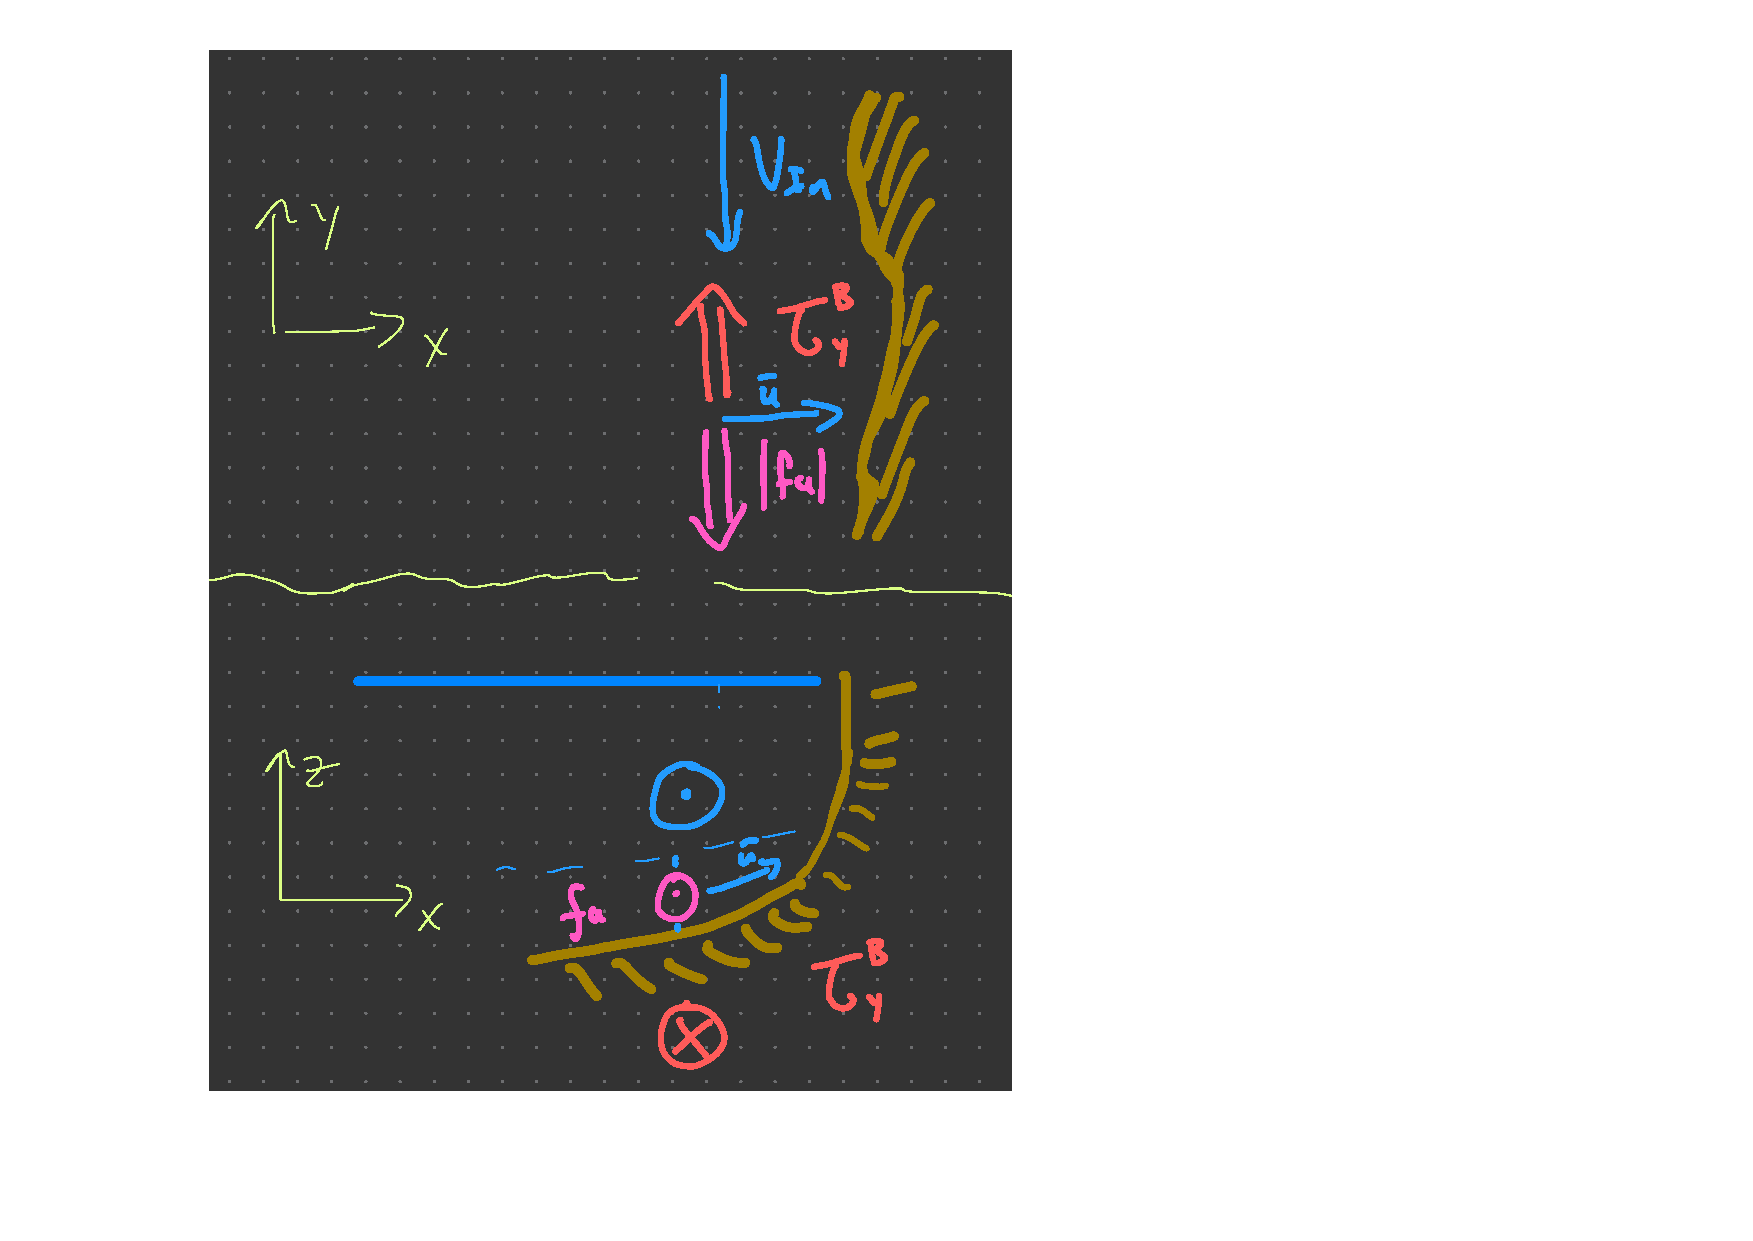
\includegraphics[width=3in]{figs/Coriolis/EkmanBottomForces}
    \caption{Sketch of the depth-integrated force balances in a bottom Ekman layer in the coastal-upwelling case. Upper is looking from above, and lower sketch is looking from the south. The bottom stress is the net stress acting to slow down the southward interior current.}
    \label{fig:EkmanBottomForces}  
  \end{center}
\end{figure}

Putting some values on these transports, usually we can estimate the windstress or bottom stress from the speed of the water or wind.  For the Oregon shelf case, the bottom stress is estimated to be something like $\tau_B^W\approx 0.1 \ \mathrm{N\,m^{-2}}$, so 
\begin{equation}
    \overline{u}D = \frac{\tau_B^W}{\rho_0 f} = \frac{0.1}{10^3 \times 10^-4} = 2\ \mathrm{m^2\,s^{-1}}
\end{equation}
where this is transport per along-shore distance.  If we average this over 20 m, then the average speed of this layer is $0.1\ \mathrm{m\,s^{-1}}$, or about 8 km/d.   We saw from the observations that dense water was seen moving up the shelf at approximately 7 km/d, so this is in agreement with our observations.  (Note that the surface mixed layer was very hard to observe in these observations so we don't make a direct comparison of its motion.)

\subsection{The Ekman spiral: fact and fiction}

Above we elided the structure of the Ekman flow and skipped to the net transport by integrating from $z=-D$ to the surface (or over the bottom Ekman layer).  The details of the Ekman flow are quite interesting, but in the end frustratingly hard to quantify and observe.

The coastal upwelling example clearly shows the effect of Ekman transport pushing water up the shelf.  However, note that the observations did not directly observe the velocity associated with this transport because the Doppler current profiler has a technical limitation near the seafloor.  So we infer the net motion from the tranport of dense water up the shelf.  I would argue that this transport is the important factor, and details of the currents in the Ekman layer are of secondary importance. 

Regardless, even elementary text books discuss the \Wikiref{Ekman spiral} which has a very idealized shape.  In this idealization, the surface currents flow at 45 degrees to the wind, and then  smoothly spirals to clockwise as it decays with depth (\fref{fig:ocean-in-motion_clip_image001}).  This ideal solution depends on a constant viscosity $\nu$ in the upper ocean.  However, that is rarely the case as the viscosity is usually a turbulent viscosity and the turbulence in the upper water column varies due to many factors.  Hence observed Ekman spirals are usually found to have more veering than predicted, and a compressed decay scale (\fref{fig:ObservedEkmanSpiral}).  

\begin{figure}[hbt]
  \begin{center}
    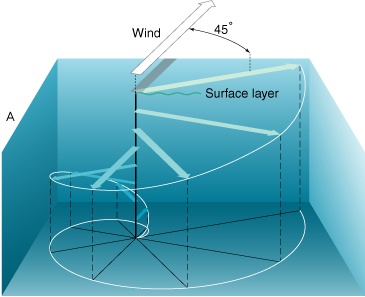
\includegraphics[width=3in]{figs/Coriolis/ocean-in-motion_clip_image001}
    \caption{Idealized Ekman spiral for flow with a constant viscosity.  \protect\url{http://oceanmotion.org/html/background/ocean-in-motion.htm}}
    \label{fig:ocean-in-motion_clip_image001}  
  \end{center}
\end{figure}

\begin{figure}[hbt]
  \begin{center}
    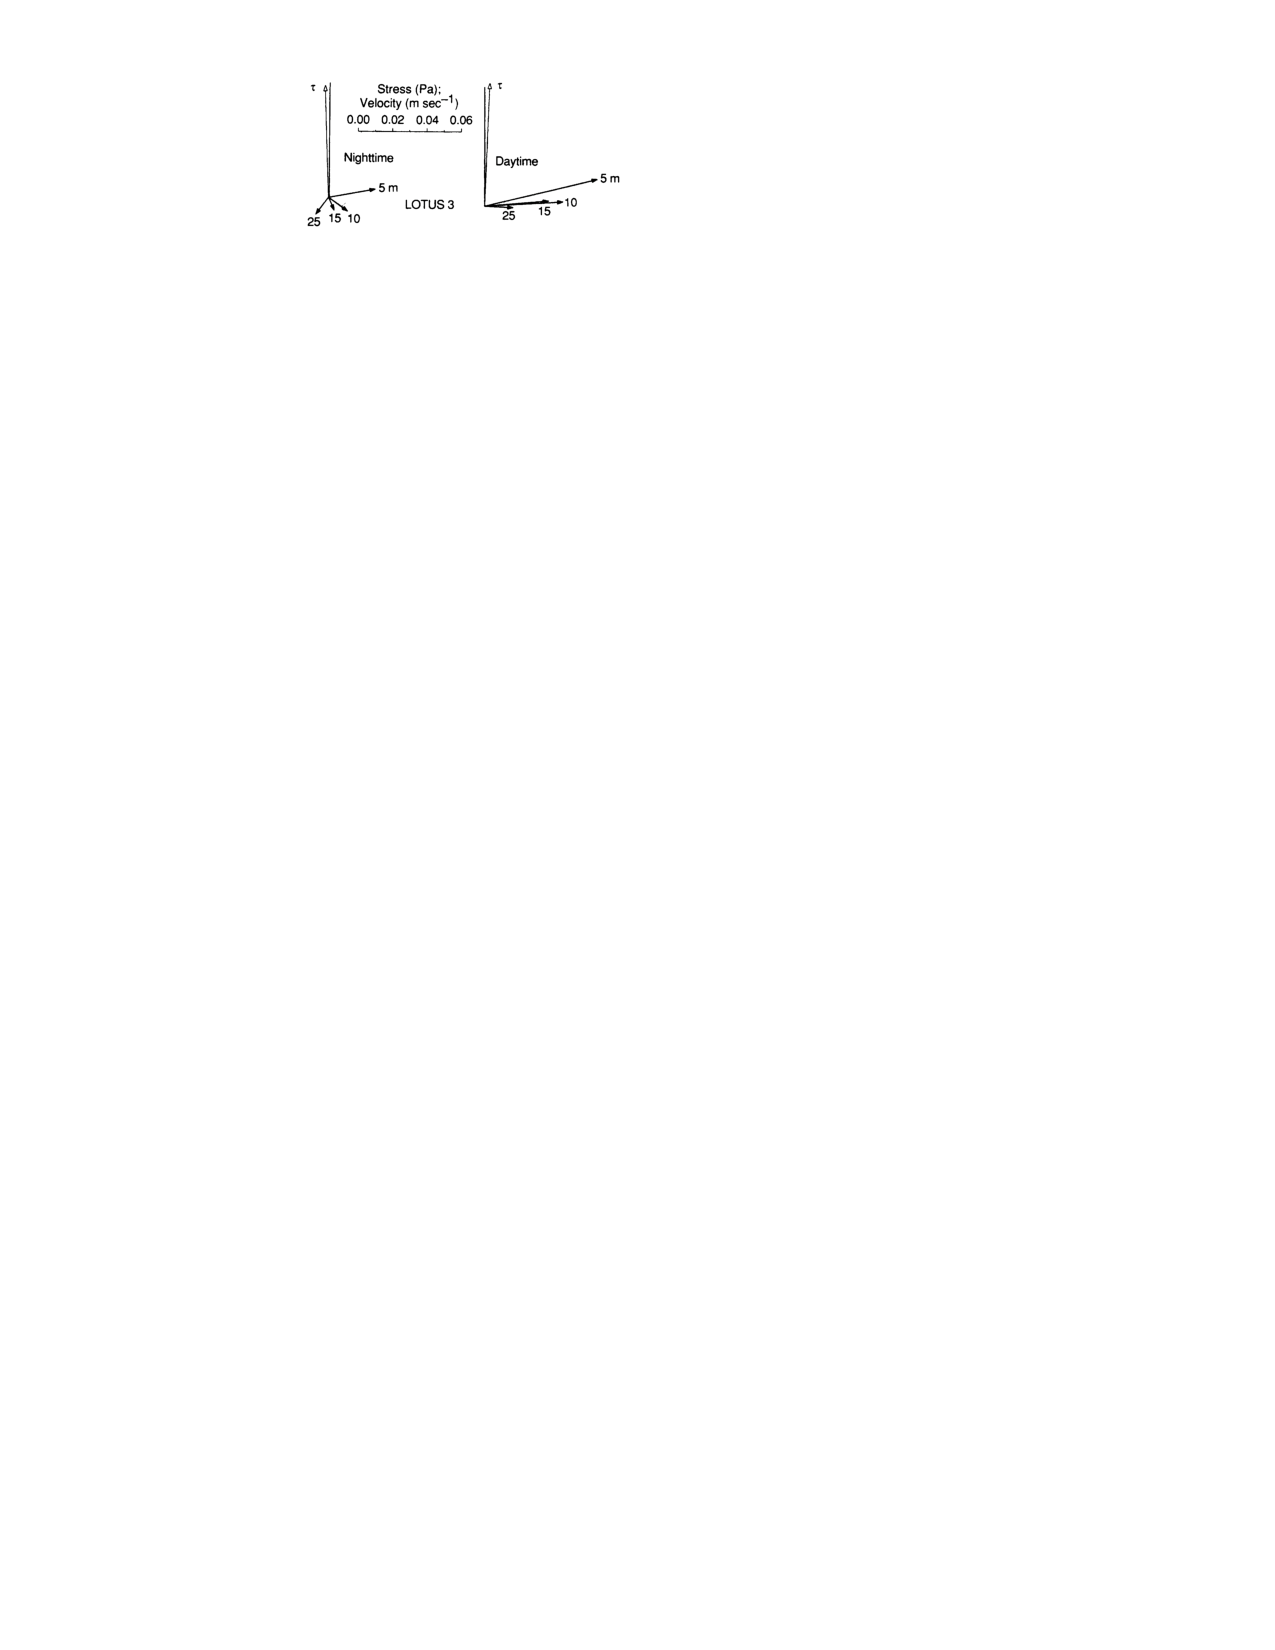
\includegraphics{figs/Coriolis/ObservedEkmanSpiral}
    \caption{Observed Ekman spiral from direct measurements in the upper ocean divided into flow at night and during the day.  Daytime stratification compresses the Ekman layer to the upper ocean.  \citep{priceetal87}}
    \label{fig:ObservedEkmanSpiral}  
  \end{center}
\end{figure}

\section{Ekman convergence and divergence}

Ekman transports tend to only affect a thin region through the upper ocean, or near the seafloor.  However, because they move water around they can make convergences and divergences.  In a convergence water piles up and then is pushed downwards, in a divergence the sea level tends to drop, and then water is pulled up from depth.  This creates pressure gradients that can then be felt from the top of the water column to the bottom.  

First, if there is a coast, steady offshore Ekman transport leads to a divergence at the coast.  This will tend to make the water level drop at the coast relative to offshore (\fref{fig:EkmanDivCoast}), until there is  replacement flow from below. It is important to remember this cross-shore pressure gradient is caused \emph{before} any replacement flow happens, and indeed this pressure gradient is what ultimately causes the replacement flow.  That there must be a replacement flow should be clear - suppose $1\ \mathrm{m^2\,s^{-1}}$ of offshore transport (see calculation above for bottom boundary layer), and suppose this is applicable 10 km offshore.  Over this 10 km, tbe water level will drop at a rate $10^{-4}\ \mathrm{m\,s^{-1}}$, or 8 m a day.  While winds clearly blow for more than a day, the sea-surface is never drawn down 8 m at the coast.  As we will see in the next chapter, the replacement flow is due to coastal upwelling in the bottom boundary layer, but there is one more step in the process that we will cover next chapter.  However, if we know the offshore transport, we can infer the vertical upwelling rate as $10^{-4}\ \mathrm{m\,s^{-1}}$.

\begin{figure}[hbt]
  \begin{center}
  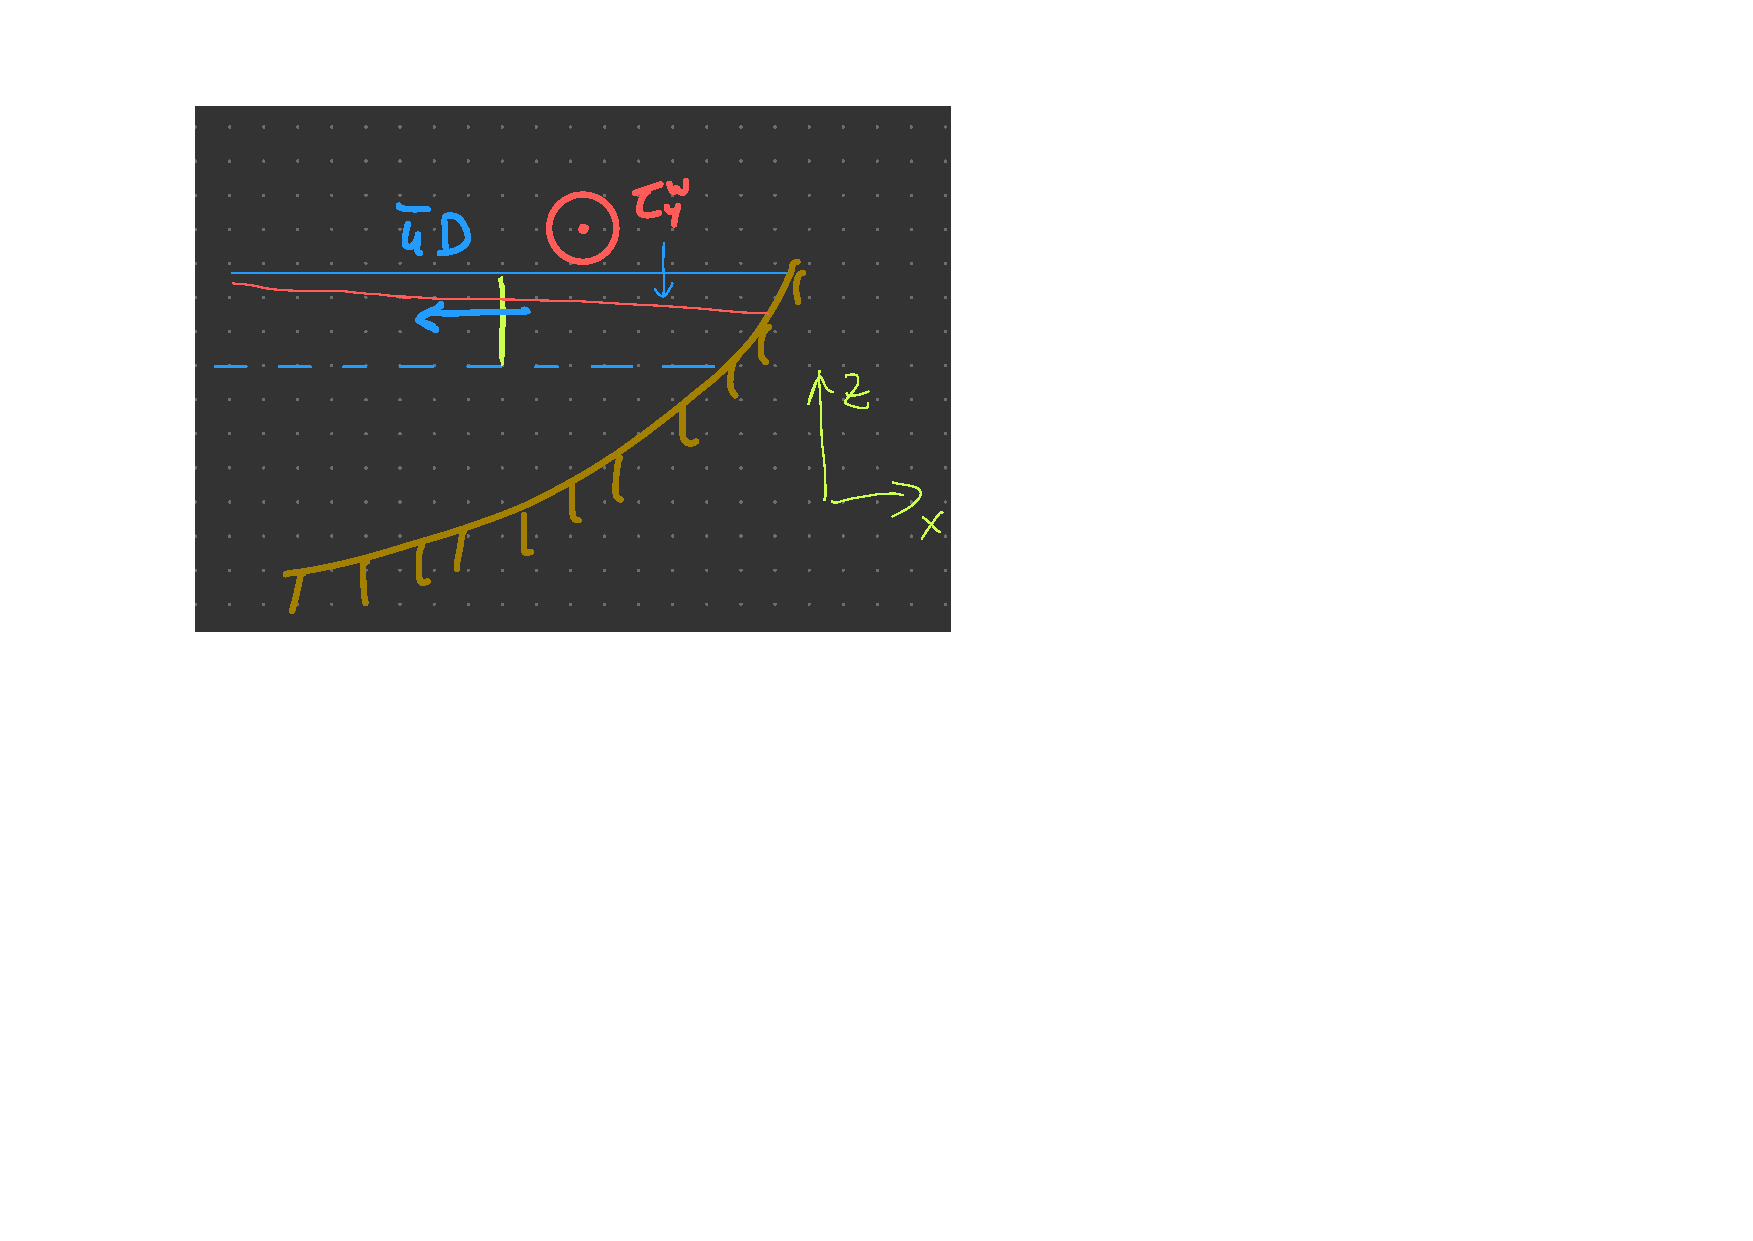
\includegraphics{figs/Coriolis/EkmanDivCoast}
    \caption{Sketch of divergence on the coast due to a southward wind ($\tau_y^w$).  Average offshore transport is everywhere except at the coast, leading to the sea surface dropping. }
    \label{fig:EkmanDivCoast}  
  \end{center}
\end{figure}

Ekman convergences and divergences are also crucially important in the interior of the ocean, away from boundaries.  In this case the convergences must be caused by changes in the wind stress. When discussing the wind-driven flow in the North Pacific, we noted that the westerlies are concentrated at 45 N, and the trades at 15 N (\fref{fig:SketchPacificConv}).  The Ekman transport in the westerlies is to the south, and in the trades it is to the north (\fref{fig:SketchPacificConv}, blue arrows), so everywhere between these two latitudes, we have an Ekman convergence or \href{https://en.wikipedia.org/wiki/Ekman_transport#Ekman_pumping}{Ekman pumping}.  The convergence causes the sea surface to be high in the middle of these winds (as observed) and drive a flow downwards.

\begin{figure}[hbt]
  \begin{center}
    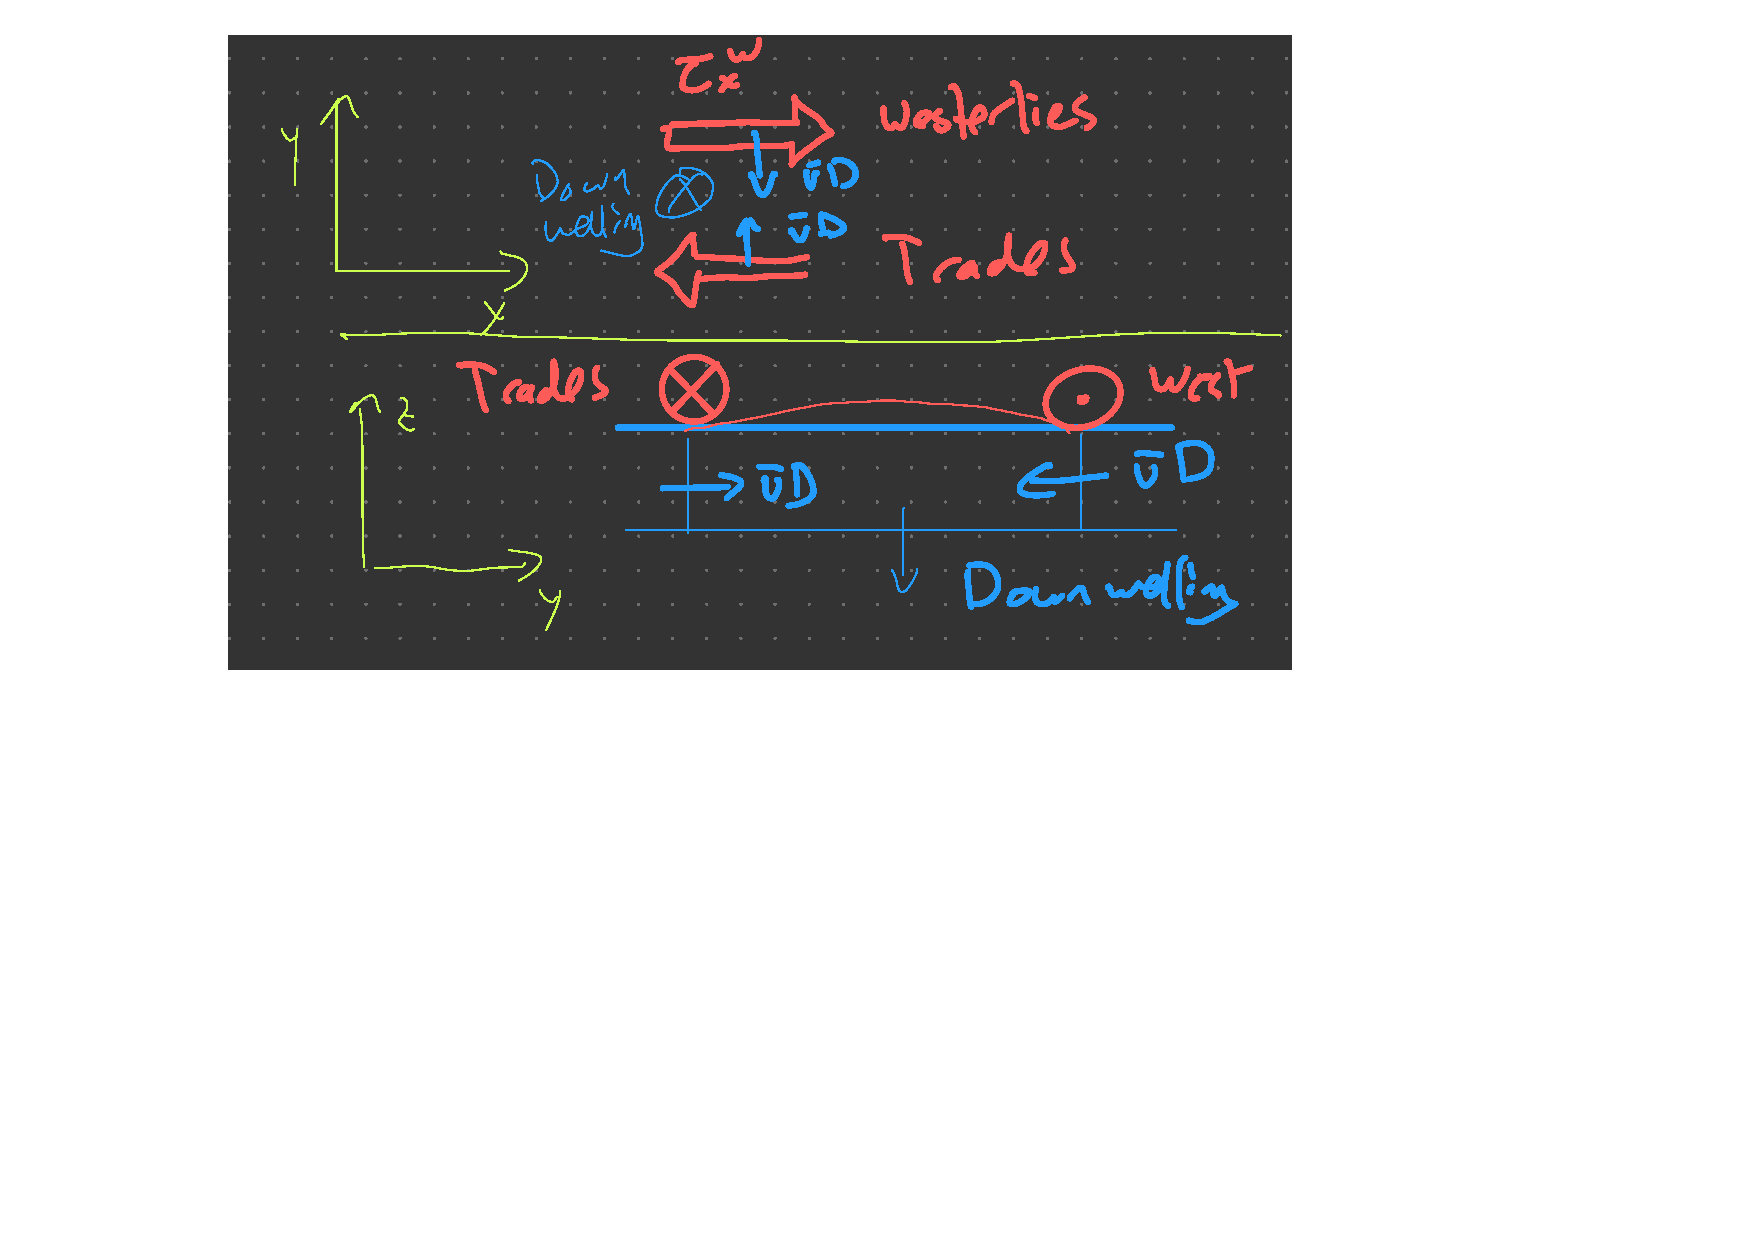
\includegraphics{figs/Coriolis/SketchPacificConv}
    \caption{Sketch of winds in the Pacific, looking from above (top) and from the east (bottom).  There is a convergence between the Westerlies and Trades (red arrows) due to the converging Ekman transports. This leads to high sea level between these latitudes, and downwelling or Ekman pumping into the interior.}
    \label{fig:SketchPacificConv}  
  \end{center}
\end{figure}

In fact, everywhere that there is a gradient in the windstress, there will either be a convergence or a divergence.  If the wind stress gradients are mostly north-south, then we can write:
\begin{equation}
    \overline{w}\ \delta y =  \overline{v}D|_{y+\delta y} - \overline{v}D|_y = - \frac{1}{\rho_0 f}\left(  \tau_x^w(y+\delta y) - \tau_x^w(y) \right)
\end{equation}
or if we allow $\delta y$ to become very small:
\begin{equation}
    w = -\frac{1}{\rho_0 f} \frac{d \tau_x^W}{d y}
\end{equation}
So in the N. Pacific, the distance between 15 and 45 N is 3300 km, so $\frac{1}{\rho_0 f}\frac{d\tau_x^W}{d y} \approx 10^{-6}\ \mathrm{ms^{-1}}$, or close to 0.1 m per day.  Integrated over the basin this represents $30\times10^{6}\ \mathrm{m^3\,s^{-1}}$.  

Note that the full Ekman vertical velocity is given by the \Wikiref{curl (mathematics)} of the  wind vector, so winds that spin in a clockwise direction tend to drive water towards the center, and winds that spin counter clockwise pull water from the center:
\begin{equation}
    \mathrm{curl} \tau^W = \frac{d \tau^W_y}{d x}-\frac{d \tau^W_x}{d y}
\end{equation}

\clearpage
\section{Exercises}

\paragraph{Coriolis to west}
Using the logic above, and a sketch, argue that shooting a hockey puck towards a target to the west (i.e. a tangential shot against the direction of rotation) will lead to a Coriolis force to the north (or towards the axis of rotation).  

\paragraph{Calculate Ekman convergence and divergence} Suppose we have a wind from the west that increases to the north so that at 30 N it blows at $0.1\ \mathrm{N\,m^2}$.  At a point 50 km north it blows at  $0.2\ \mathrm{N\,m^2}$, and 100 km north it blows at  $0.3\ \mathrm{N\,m^2}$. What is the average rate of Ekman ``pumping'' between the wind measurements (in m/s)? Sketch.

\paragraph{Where is the Ekman pumping in N. Pacific?}

Based on the figure below, where is there Ekman pumping and suction (by latitude) in the North Pacific? How well does this correspond to the shape of the isohalines of the upper ocean in the salinity section below?

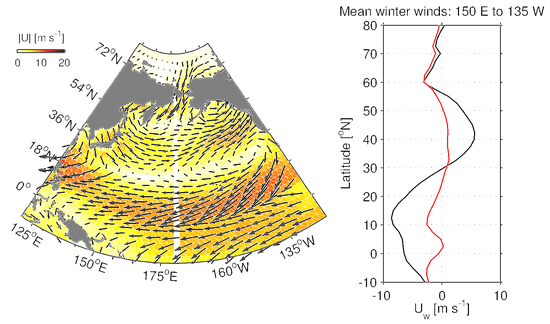
\includegraphics{figs/Coriolis/PacificWindsSm}
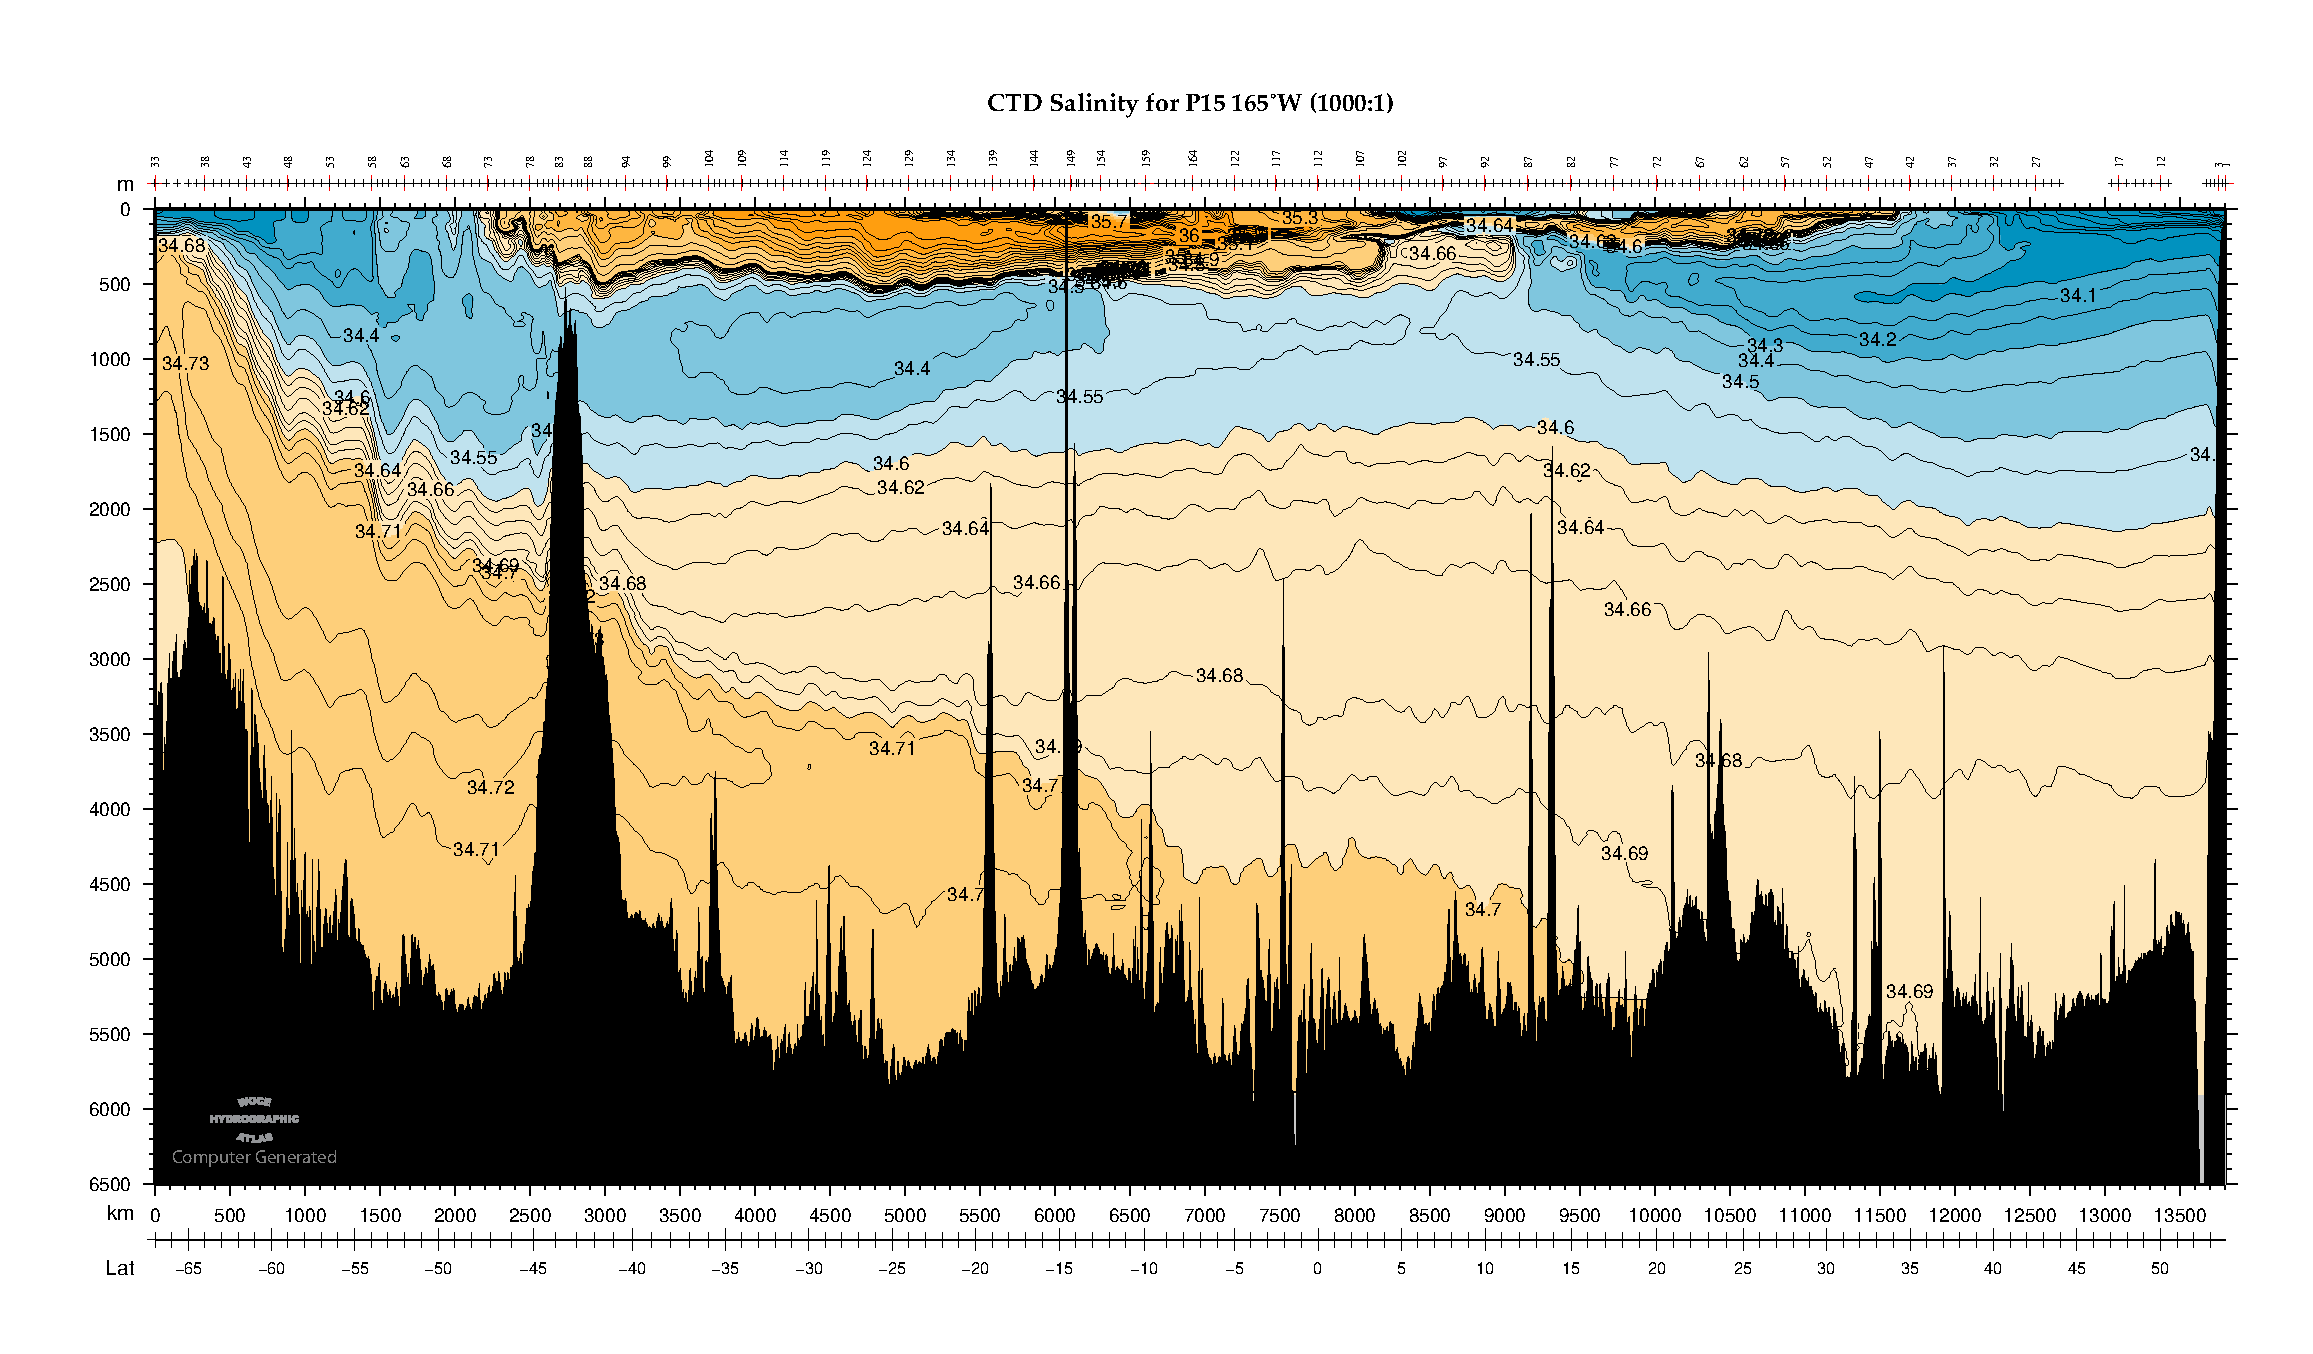
\includegraphics{figs/WaterMasses/P15_CTDSAL_all_1000}

%%% Local Variables:
%%% mode: latex
%%% TeX-master: t
%%% End:
